\documentclass[UTF8,a4paper,11pt]{ctexart}
\usepackage[margin=2.4cm]{geometry}
\usepackage{graphicx}
\usepackage{booktabs}
\usepackage{longtable}
\usepackage{array}
\usepackage{hyperref}
\usepackage{float}
\graphicspath{{../../}{}}
\hypersetup{colorlinks=true,linkcolor=blue,urlcolor=blue}
\title{报告数据与数据分析部分}
\author{自动整理自项目中文报告}
\date{\today}
\begin{document}
\maketitle
\tableofcontents
\newpage
\section{基础几何等价性报告：数据与数据分析}
\noindent\textbf{来源文件：}reports/zh/大报告\_中文\_完整版\_改写版.docx

\subsection{第二部分　度量方法}

\subsubsection{2.1　性能指标：MSE}

衡量预测准不准，用均方误差：

变体：NN\_mse\_vs\_y（NN vs 真值）、FPR\_mse\_vs\_y（FullPR vs 真值）、FPR\_mse\_vs\_NN（FullPR vs NN 输出）、LTPR\_mse\_vs\_NN（LTPR vs NN 输出）。后两者以 NN 输出为“真值”，因为关心的是“像不像 NN”。新增的 NN 基准指标包括：*\_mse\_delta\_vs\_NN（模型 MSE 减 NN MSE，负值表示模型更准）、*\_improve\_vs\_NN\_pct（相对 NN 的改善百分比，正值表示模型更好）、*\_better\_than\_NN（该 run 是否击败 NN）。

\subsubsection{2.2　性能差距：abs\_rmse\_gap}

取平方根（化为 RMSE，与数据同量纲）再取绝对差。越小说明两模型准确度越接近。

\subsubsection{2.3　几何指标：形状距离（核心创新）}

不只比“准不准”，更比两个模型学到的函数“长得像不像”。做法：把每个模型在测试点的预测与输入拼成响应曲面上的点云。对模型 A：

两片点云输入坐标相同，仅预测维不同。用 Procrustes 分析对齐------平移、缩放、旋转------再算逐点残差平方和：

它模掉了平移/旋转/缩放，衡量纯粹的“形状像不像”。接近 0=形状几乎相同。这与 MSE 不同：曲面平移一个常数，形状距离不变而 MSE 会变，两者捕捉不同信息。

图中的形状距离：shape\_NN\_FPR\_in（数据区内）、shape\_NN\_FPR\_ext（外推区）、shape\_NN\_LTPR（NN 与 LTPR）、shape\_LTPR\_FPR（两种多项式之间）。

\subsubsection{2.4　激活改变量：act\_io\_sum}

量化激活注入了多少非线性。对每个激活层，用形状距离测 u$\to$g(u) 的“弯曲”，对所有激活层加总得 act\_io\_scaled\_sum（输入归一化到 [-1,1]）。激活近似直线$\to$网络近线性$\to$近低阶多项式；激活强烈弯曲$\to$注入大量非线性。这是最初假设的自变量。

\subsubsection{2.5　实验设计}

数据集 5 个：paper\_poly3（3 阶，3 隐层时命中，作 well-specified 对照）、paper\_poly4（4 阶，严格欠设定）、smooth\_nonlinear（固定频率非多项式）、smooth\_nonlinear\_rand（随机频率非多项式，最严格）。激活 3 种（softplus/tanh/sigmoid），深度 3 种（4 / 8,4 / 16,8,4），每配置固定数据、扫 50 个网络初始化 seed（论文式重复），共约 3000 次模拟。

\subsection{第三部分　实验图表全解}

本部分嵌入全部 9 张结果图（4 数据集 $\times$ 几何图/MSE图，加总览箱线图），并逐子图解读。所有散点图中每点为一次模拟，颜色=激活函数（绿 softplus / 橙 tanh / 深蓝 sigmoid）。

\subsubsection{3.1　几何图通用结构（11 子图）}

子图(1)(2)　act-change $\to$ NN-FullPR 数据区接近度（缩放/未缩输入）：激活注入非线性越多，NN 与多项式数据区内越不像吗？

子图(3)　act-change $\to$ 外推接近度：常现水平条带=饱和激活外推时与多项式系统性偏离。

子图(4)　act-change $\to$ 性能差距：激活改变能否直接预测性能差。

子图(5)　相邻层非线性 $\to$ 数据区接近度：(1)的交叉验证。

子图(6)　NN-FullPR 接近度 $\to$ 性能差距（核心）：呈上升带即证明几何近$\Rightarrow$性能近。

子图(7)　NN-LTPR 接近度 $\to$ 性能差距：泰勒翻译与 NN 像不像、能否预测性能差。

子图(8)　act-change $\to$ NN-LTPR 接近度：激活改变越大泰勒越易偏离 NN（泰勒失效征兆）。

子图(9)　NN-LTPR vs NN-FullPR 接近度：两种多项式代理是否一致。

子图(10)(11)　LTPR-FullPR 接近度 $\to$ 性能差距 / vs NN-FullPR：两种多项式彼此关系。

\subsubsection{3.2　MSE 图通用结构（6 子图）}

子图(1)　act-change $\to$ NN 自身 MSE：激活非线性是否影响 NN 拟合质量。

子图(2)　NN-FullPR 接近度 $\to$ FullPR 复刻 NN 的 MSE：通常干净正相关直线，验证形状距离有效。

子图(3)　NN-LTPR 接近度 $\to$ LTPR 复刻 NN 的 MSE：注意 LTPR 偶尔爆炸到 1e8（泰勒失效）。

子图(4)　NN MSE vs FullPR MSE（y=x 线）：点在线下=FullPR 更准，线上=NN 更准。新加入的 nn\_baseline 图把这个判断汇总为胜率和中位改善，更适合报告“哪个更好”。

子图(5)　FullPR vs LTPR 复刻 NN 的 MSE：两种多项式对比，LTPR 爆炸在此显现。

子图(6)　NN MSE $\to$ NN-FullPR 性能差距：NN 拟合好坏是否影响它与多项式的接近度。

\subsubsection{3.3　数据集 1：paper\_poly4（4 阶，严格欠设定）}

数据由 4 阶多项式生成，网络最深 3 层、Full-PR 最高 3 阶，多项式无法恰好命中------检验欠设定情形的主力。

\paragraph{几何图}

3.3　数据集 1：paper\_poly4（4 阶，严格欠设定） --- 几何距离 vs 接近度/性能（11 子图）

这张几何图上看到了什么：

\begin{itemize}
\item 子图(6)（核心）：清晰上升带，分成几簇，右上高距离高差距簇对应较深网络------核心命题成立。
\end{itemize}

\begin{itemize}
\item 子图(1)(2)：点云水平偏散，数据区内激活改变不能很好预测接近度。
\end{itemize}

\begin{itemize}
\item 子图(3)：右上一个 softplus 离群点冲到 0.8，个别 run 外推严重偏离。
\end{itemize}

\begin{itemize}
\item 子图(7)(8)(9)(10)(11)（LTPR）：横轴 shape\_NN\_LTPR 多数贴 0（复刻好），少数拖到 0.8+ 是泰勒偏离的 run。
\end{itemize}

\paragraph{MSE 图}

3.3　数据集 1：paper\_poly4（4 阶，严格欠设定） --- 各指标 vs MSE 及模型间对比（6 子图）

这张 MSE 图上看到了什么：

\begin{itemize}
\item 子图(2)：极干净正相关直线，分三段（三种深度），强力验证形状距离预测复刻误差。
\end{itemize}

\begin{itemize}
\item 子图(3)：纵轴标到 4$\times$10$^5$------LTPR 偶尔灾难性爆炸，绝大多数贴底为 0。
\end{itemize}

\begin{itemize}
\item 子图(4)（y=x 线）：点多在对角线附近及下方，FullPR 略占优的情形不少。
\end{itemize}

\begin{itemize}
\item 子图(6)：分叉弧形结构，反映不同深度/收敛状态的子群。
\end{itemize}

\paragraph{清洗后图（剔除未收敛 NN 与 LTPR 失效值后重绘）}

下方为运行 analyze\_results.py 后的清洗版结果：剔除组内 NN\_mse 超过中位数 10 倍的未收敛 run，并将 LTPR\_mse\_vs\_NN 超过 100 的样本标记为失效（LTPR 相关子图中排除，单独在失效图中展示）。

3.3　数据集 1：paper\_poly4 --- 清洗后核心几何与性能关系

\begin{itemize}
\item 核心子图（NN-FullPR 接近度 $\to$ 性能差距）清洗后呈现两簇更干净的上升弧线，离群（未收敛）run 已剔除，几何近$\Rightarrow$性能近的结构比原图更清晰。
\end{itemize}

3.3　数据集 1：paper\_poly4 --- LayerTaylor-PR 失效尾部（log 轴）

\begin{itemize}
\item 失效尾部峰值约 6$\times$10$^5$，与清洗前数据一致；多数点仍贴近 1e-4 量级，说明逐层泰勒展开在多数情形下能精确复刻 NN。
\end{itemize}

\subsubsection{3.4　数据集 2：paper\_poly3（3 阶，3 隐层时命中）}

数据由 3 阶多项式生成，3 隐层时 Full-PR 阶数正好等于数据阶数，是 well-specified 对照组。

\paragraph{几何图}

3.4　数据集 2：paper\_poly3（3 阶，3 隐层时命中） --- 几何距离 vs 接近度/性能（11 子图）

这张几何图上看到了什么：

\begin{itemize}
\item 整体纵轴量级比 poly4 小一个数量级（形状距离最大约 0.014），命中后两模型都很准、几何更贴近。
\end{itemize}

\begin{itemize}
\item 子图(6)（核心）：呈“拱形+上升”------低距离区先有命中导致的极小差距拱形，再随距离上升。
\end{itemize}

\begin{itemize}
\item 子图(3)：纵轴到 0.035，命中时连外推都较一致。
\end{itemize}

\begin{itemize}
\item 子图(8)：可见激活改变越大、LTPR 越易偏离 NN 的弱趋势。
\end{itemize}

\paragraph{MSE 图}

3.4　数据集 2：paper\_poly3（3 阶，3 隐层时命中） --- 各指标 vs MSE 及模型间对比（6 子图）

这张 MSE 图上看到了什么：

\begin{itemize}
\item 子图(2)：干净正相关直线，量级很小（到 0.012）。
\end{itemize}

\begin{itemize}
\item 子图(3)：纵轴到约 900------仍有 LTPR 失效，但比 poly4 爆炸量级小得多。
\end{itemize}

\begin{itemize}
\item 子图(4)（y=x 线）：多数点贴近原点，命中使两模型都很准、差距很小。
\end{itemize}

\begin{itemize}
\item 子图(6)：分叉弧形，结构类似 poly4 但尺度更小。
\end{itemize}

\paragraph{清洗后图（剔除未收敛 NN 与 LTPR 失效值后重绘）}

下方为运行 analyze\_results.py 后的清洗版结果：剔除组内 NN\_mse 超过中位数 10 倍的未收敛 run，并将 LTPR\_mse\_vs\_NN 超过 100 的样本标记为失效（LTPR 相关子图中排除，单独在失效图中展示）。

3.4　数据集 2：paper\_poly3 --- 清洗后核心几何与性能关系

\begin{itemize}
\item 核心关系呈现清晰的“低距离拱形 + 整体上升”结构，命中阶数（3 隐层）时差距极小，验证 well-specified 情形下的退化路径。
\end{itemize}

3.4　数据集 2：paper\_poly3 --- LayerTaylor-PR 失效尾部（log 轴）

\begin{itemize}
\item 失效尾部峰值约 900，比 paper\_poly4 小约 3 个数量级，与“命中阶数时退化路径更短、泰勒展开更稳定”的直觉一致。
\end{itemize}

\subsubsection{3.5　数据集 3：smooth\_nonlinear（固定频率非多项式，仅 softplus）}

真值是固定频率 sin 类非多项式，多项式永远无法精确表示------严格欠设定。仅跑 softplus，故只有绿点。

\paragraph{几何图}

3.5　数据集 3：smooth\_nonlinear（固定频率非多项式，仅 softplus） --- 几何距离 vs 接近度/性能（11 子图）

这张几何图上看到了什么：

\begin{itemize}
\item 存在极端离群 run：子图(1)(4)(6)(7)(10)里都有孤点冲到 perf gap$\approx$8.6 或形状距离$\approx$0.84------NN 训练崩溃，应剔除。
\end{itemize}

\begin{itemize}
\item 子图(6)（核心）：除去离群点，主体仍清晰上升带，几何近$\Rightarrow$性能近成立。
\end{itemize}

\begin{itemize}
\item 子图(3)：点分布在 0.1--0.3 带状区，外推差距明显大于 poly 系列（非多项式真值更难外推一致）。
\end{itemize}

\begin{itemize}
\item 子图(8)：明显正相关云------激活改变越大 LTPR 越偏离 NN，泰勒失效的清晰证据。
\end{itemize}

\paragraph{MSE 图}

3.5　数据集 3：smooth\_nonlinear（固定频率非多项式，仅 softplus） --- 各指标 vs MSE 及模型间对比（6 子图）

这张 MSE 图上看到了什么：

\begin{itemize}
\item 子图(1)(3)(5)(6)都有 NN\_mse$\approx$73 的极端点------同一崩溃 run，横轴被拉长。
\end{itemize}

\begin{itemize}
\item 子图(3)：纵轴到 6$\times$10$^4$，LTPR 失效尾部明显。
\end{itemize}

\begin{itemize}
\item 子图(5)：LTPR 纵轴爆到数万，FullPR 始终贴 0，对比鲜明。
\end{itemize}

\begin{itemize}
\item 子图(4)（y=x 线）：除崩溃点外贴近原点，softplus 下两模型都较准。
\end{itemize}

\paragraph{清洗后图（剔除未收敛 NN 与 LTPR 失效值后重绘）}

下方为运行 analyze\_results.py 后的清洗版结果：剔除组内 NN\_mse 超过中位数 10 倍的未收敛 run，并将 LTPR\_mse\_vs\_NN 超过 100 的样本标记为失效（LTPR 相关子图中排除，单独在失效图中展示）。

3.5　数据集 3：smooth\_nonlinear --- 清洗后核心几何与性能关系

\begin{itemize}
\item 剔除 NN\_mse$\approx$73 的崩溃 run 后，核心上升带清晰可见；该数据集仅跑 softplus 激活（图例中 tanh/sigmoid 无点属预期，非数据缺失）。
\end{itemize}

3.5　数据集 3：smooth\_nonlinear --- LayerTaylor-PR 失效尾部（log 轴）

\begin{itemize}
\item 失效尾部峰值约 6$\times$10$^4$；act\_io\_scaled\_sum 越大、LTPR 越易失效的正相关趋势在 log 图中清晰可见。
\end{itemize}

\subsubsection{3.6　数据集 4：smooth\_nonlinear\_rand（随机频率非多项式，最严格）}

真值是随机频率/相位 sin 类函数，每次目标都不同，最严格欠设定，三种激活全测。检验普适性的关键。

\paragraph{几何图}

3.6　数据集 4：smooth\_nonlinear\_rand（随机频率非多项式，最严格） --- 几何距离 vs 接近度/性能（11 子图）

这张几何图上看到了什么：

\begin{itemize}
\item 子图(6)（核心）：非常漂亮的上升带，三种激活混在同一条带------几何近$\Rightarrow$性能近在最严格场景下普适成立。
\end{itemize}

\begin{itemize}
\item 子图(3)：清晰水平条带（约 0.75/0.5/0.2），尤其 tanh/sigmoid------饱和激活外推偏离多项式的典型指纹。
\end{itemize}

\begin{itemize}
\item 子图(1)(2)：低 act 区先升、高 act 区散开，关系复杂非单调。
\end{itemize}

\begin{itemize}
\item 子图(7)(10)：丰富带状结构，LTPR 在此数据集多数有效（横轴到 1.0）。
\end{itemize}

\paragraph{MSE 图}

3.6　数据集 4：smooth\_nonlinear\_rand（随机频率非多项式，最严格） --- 各指标 vs MSE 及模型间对比（6 子图）

这张 MSE 图上看到了什么：

\begin{itemize}
\item 子图(2)：教科书级正相关直线，三种激活完全重合在一条线上。
\end{itemize}

\begin{itemize}
\item 子图(3)：纵轴到 3$\times$10$^8$------本数据集 LTPR 爆炸最严重，泰勒失效最极端的证据。
\end{itemize}

\begin{itemize}
\item 子图(4)（y=x 线）：点在对角线两侧水平带上（FullPR 离散取值造成横带），NN 与 FullPR 互有胜负。
\end{itemize}

\begin{itemize}
\item 子图(6)：独特“X 形”双分支结构，对应两类收敛模式，值得专门分析。
\end{itemize}

\paragraph{清洗后图（剔除未收敛 NN 与 LTPR 失效值后重绘）}

下方为运行 analyze\_results.py 后的清洗版结果：剔除组内 NN\_mse 超过中位数 10 倍的未收敛 run，并将 LTPR\_mse\_vs\_NN 超过 100 的样本标记为失效（LTPR 相关子图中排除，单独在失效图中展示）。

3.6　数据集 4：smooth\_nonlinear\_rand --- 清洗后核心几何与性能关系

\begin{itemize}
\item 三种激活函数的核心上升带清洗后几乎完全重合，是“几何近$\Rightarrow$性能近”在最严格设定下普适成立的最强证据。
\end{itemize}

3.6　数据集 4：smooth\_nonlinear\_rand --- LayerTaylor-PR 失效尾部（log 轴）

\begin{itemize}
\item 失效尾部峰值约 3$\times$10$^8$，是四个数据集中最极端的爆炸，印证随机频率目标对泰勒收敛域的破坏最为严重。
\end{itemize}

\subsubsection{3.7　总览箱线图（所有数据集、所有重复）}

箱线图：箱体=中间50\%数据，箱中横线=中位数，须=正常范围，须外圆圈=离群点。

三种激活下三个关键量的分布

三个子图：

\begin{itemize}
\item 左（激活改变总量）：中位数都在 0.2--0.25；sigmoid 箱体和上须最长（变异最大），tanh 最紧凑。
\end{itemize}

\begin{itemize}
\item 中（NN-FullPR 数据区形状距离）：三种激活箱体都极度贴 0------绝大多数情况 NN 与多项式很像；但都拖大量向上离群圈（softplus 到 0.83）。
\end{itemize}

\begin{itemize}
\item 右（性能差距）：箱体贴地、拖离群点（softplus 有 8.5 的极端值=崩溃 run）。
\end{itemize}

关键提醒：离群圈都指向同一类问题------未收敛训练与泰勒失效。结论应基于箱体主体，离群点需单独处理。

\subsection{第四部分　定量发现}

\subsubsection{4.0　以 NN 为基准的模型胜负}

除了“形状是否接近”和“性能是否接近”，本次新增图表还直接比较各模型相对 NN 的预测优劣。判断规则是：若某模型的 MSE vs y 小于 NN\_mse\_vs\_y，则该 run 中该模型胜过 NN。nn\_baseline 图左侧给出胜率，右侧给出相对 NN 的中位改善百分比；50\% 和 0\% 分别是胜负分界线。

\begin{longtable}{p{0.237\textwidth}p{0.237\textwidth}p{0.237\textwidth}p{0.237\textwidth}}
\toprule
模型 & 有效 run & 相对 NN 胜率 & 中位改善 \\
\midrule
\endfirsthead
\toprule
模型 & 有效 run & 相对 NN 胜率 & 中位改善 \\
\midrule
\endhead
FullPR & 2960 & 38.9\% & -85.3\% \\
Taylor-PR & 982 & 0.0\% & -143955.8\% \\
LayerTaylor-PR & 2960 & 5.6\% & -1392.6\% \\
\bottomrule
\end{longtable}

总体看，FullPR 是唯一真正能和 NN 正面对打的模型，但全体合并后胜率为 38.9\%、中位改善为 -85.3\%，说明 NN 更稳。Taylor-PR 胜率为 0\%，LayerTaylor-PR 总体胜率仅 5.6\%，二者的主要价值是解释和复刻 NN，而不是击败 NN。

\emph{图：paper\_poly3 的 NN 基准胜负图。FullPR 多数时候胜过 NN。}

\emph{图：paper\_poly4 的 NN 基准胜负图。NN 在该欠设定高阶任务中更稳。}

\emph{图：smooth\_nonlinear 的 NN 基准胜负图。FullPR 略优于 NN。}

\emph{图：smooth\_nonlinear\_rand 的 NN 基准胜负图。NN 优势最明显。}

分数据集结论：paper\_poly3 和 smooth\_nonlinear 中，FullPR 更常胜过 NN；paper\_poly4 和 smooth\_nonlinear\_rand 中，NN 更稳。这说明“神经网络可被多项式解释”与“多项式一定更准”是两个不同命题。几何等价性描述的是形状和性能差距之间的规律，预测胜负还取决于真函数阶数、随机非线性、特征族是否匹配以及训练稳定性。

基于 3000 次重复模拟，Spearman 秩相关结果（* 表示 p<0.05）。这是本研究的量化核心。

\subsubsection{4.1　核心命题：几何接近度 $\to$ 性能接近度}

NN-FullPR 形状距离与性能差距的相关性，是项目基石：

\begin{longtable}{p{0.237\textwidth}p{0.237\textwidth}p{0.237\textwidth}p{0.237\textwidth}}
\toprule
数据集 & Spearman $\rho$ & p 值 & n \\
\midrule
\endfirsthead
\toprule
数据集 & Spearman $\rho$ & p 值 & n \\
\midrule
\endhead
全体 ALL & 0.840* & $\approx$ 0 & 3000 \\
paper\_poly4 & 0.873* & 1.4e-281 & 900 \\
paper\_poly3 & 0.836* & 3.4e-236 & 900 \\
smooth\_nonlinear & 0.848* & 3.7e-84 & 300 \\
smooth\_nonlinear\_rand & 0.443* & 1.2e-44 & 900 \\
\bottomrule
\end{longtable}

结论：无论命中、欠设定、还是非多项式真值，几何接近度都强烈、显著地预测性能接近度。这在数学上并非自动成立（形状距离模掉缩放），因此是有内容的经验规律，而非恒等式。

\subsubsection{4.2　激活影响主要在外推}

激活改变（缩放）与接近度/性能的相关性：

\begin{longtable}{p{0.280\textwidth}p{0.280\textwidth}p{0.280\textwidth}}
\toprule
关系 & 全体 $\rho$ & 解读 \\
\midrule
\endfirsthead
\toprule
关系 & 全体 $\rho$ & 解读 \\
\midrule
\endhead
$\to$ 数据区接近度 & 0.172* & 数据区内关系弱 \\
$\to$ 外推接近度 & 0.556* & 激活影响主要在外推 \\
$\to$ 性能差距 & 0.017 & 几乎无直接关系（中间隔着几何） \\
相邻层非线性 $\to$ 数据区接近度 & 0.523* & 另一非线性度量给出中等正相关 \\
\bottomrule
\end{longtable}

饱和激活（tanh/sigmoid）外推时趋平、多项式发散，差距锁定成固定值，在子图(3)形成水平条带。

\subsubsection{4.3　辛普森悖论：最初假设的修正}

“激活改变小$\to$更接近多项式”这一最初假设，在合并数据上呈正相关（+0.17），但在每个数据集内部却是负相关：

\begin{longtable}{p{0.280\textwidth}p{0.280\textwidth}}
\toprule
数据集 & act-change $\to$ 数据区接近度 $\rho$ \\
\midrule
\endfirsthead
\toprule
数据集 & act-change $\to$ 数据区接近度 $\rho$ \\
\midrule
\endhead
paper\_poly4 & -0.465* \\
paper\_poly3 & -0.283* \\
smooth\_nonlinear\_rand & -0.252* \\
smooth\_nonlinear & -0.494* \\
\bottomrule
\end{longtable}

合并时的正号是组间差异制造的假象（辛普森悖论）。教训：必须分数据集报告，这也是全程分图的原因。

\subsubsection{4.4　逐层泰勒展开的灾难性失效}

LTPR 通过泰勒级数把网络翻译成多项式：

仅当 u 在收敛域内有效。突触电位过大时高次项 u\textasciicircum{}k 爆炸、多项式发散，预测可达 1e8，而 NN 输出仅 0.00x 量级。这是稀有但灾难性的失效：多数 run 完美复刻（误差 1e-9），偶尔彻底爆炸。各数据集 LTPR MSE 失效尾部峰值：paper\_poly3 约 900，paper\_poly4 约 4$\times$10$^5$，smooth\_nonlinear 约 6$\times$10$^4$，smooth\_nonlinear\_rand 约 3$\times$10$^8$。这精确印证 Morala (2021) 关于泰勒近似收敛边界的核心警告。

\section{测度加权采样大实验：数据与数据分析}
\noindent\textbf{来源文件：}reports/zh/大报告\_中文\_完整版\_测度加权大实验更新版.docx

\subsection{1. 实验流程}

实际应用中无法预先知道 NN 与 FullPR/TYPR 是否接近。因此实验先在训练集上做均匀 pilot 抽样，训练初始 NN，再计算该 NN 与 FullPR、TYPR 的响应曲面距离。距离经过归一化后转成下一批数据中的 D-optimal 比例。

\begin{figure}[htbp]
\centering
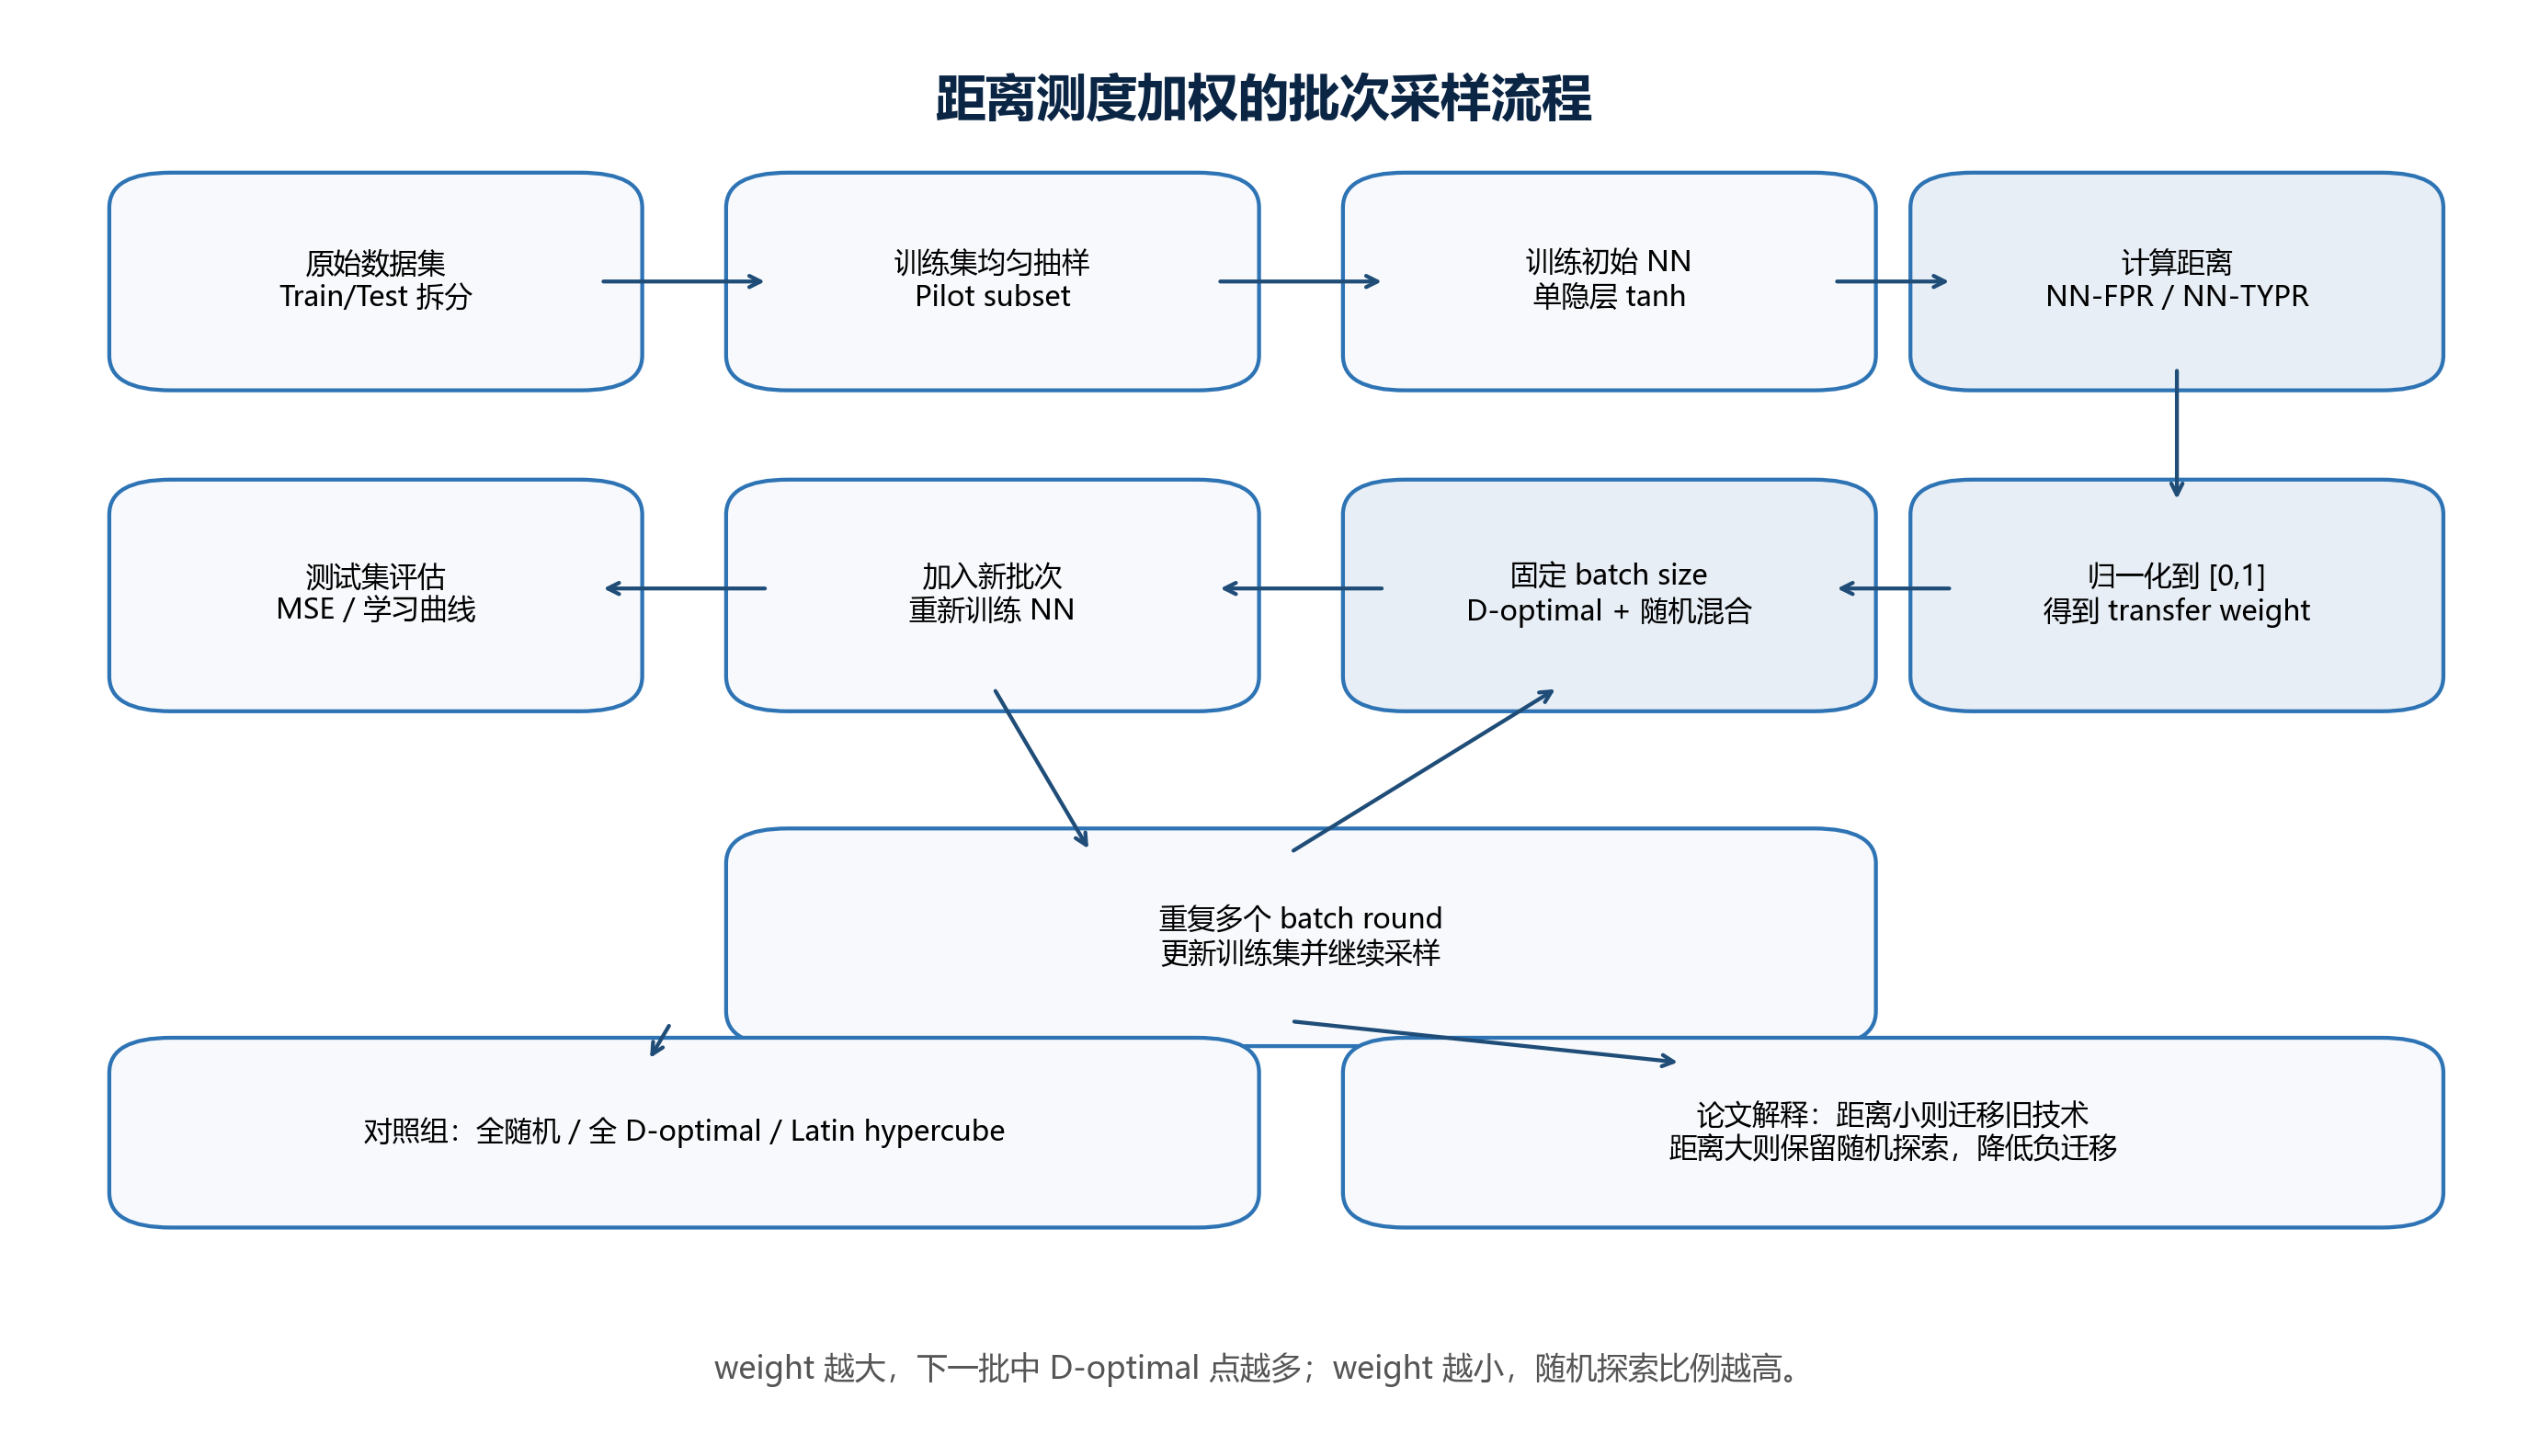
\includegraphics[width=0.92\textwidth]{figures/measure_weighted/measure_weighted_sampling_flowchart_cn.png}
\caption{距离测度加权的批次采样流程}
\end{figure}

\subsection{2. 实验设计}

\begin{enumerate}
\item 对每个数据集做 75/25 train/test 拆分，训练集内先均匀抽取 5\% 作为 pilot subset。
\end{enumerate}

\begin{enumerate}
\item 用 pilot subset 训练单隐层 tanh NN；在 pilot validation 上计算 NN-FPR 和 NN-TYPR 距离。
\end{enumerate}

\begin{enumerate}
\item 主实验使用 mean(d\_FPR, d\_TYPR) 而不是 min(...)，避免高维下单个 PR 代理偶然贴近导致过度使用 D-optimal。
\end{enumerate}

\begin{enumerate}
\item 每轮固定新增 500 点，Measure-weighted 策略按 weight 混合 D-optimal 点和随机点；对照组为全随机、全 D-optimal 和 Latin hypercube。
\end{enumerate}

\subsection{3. 主结果}

\begin{longtable}{p{0.158\textwidth}p{0.158\textwidth}p{0.158\textwidth}p{0.158\textwidth}p{0.158\textwidth}p{0.158\textwidth}}
\toprule
p & 策略 & Final MSE & 相对随机提升 & 正提升率 & 运行数 \\
\midrule
\endfirsthead
\toprule
p & 策略 & Final MSE & 相对随机提升 & 正提升率 & 运行数 \\
\midrule
\endhead
20 & Latin hypercube & 0.004811 & 5.79\% & 76.0\% & 50 \\
20 & D-optimal & 0.004986 & 4.11\% & 76.0\% & 50 \\
20 & Measure-weighted & 0.004993 & 4.40\% & 72.0\% & 50 \\
20 & Random & 0.005113 & 0.00\% & 0.0\% & 50 \\
50 & Latin hypercube & 0.018574 & 0.17\% & 46.0\% & 50 \\
50 & Random & 0.018808 & 0.00\% & 0.0\% & 50 \\
50 & Measure-weighted & 0.019143 & 0.50\% & 54.0\% & 50 \\
50 & D-optimal & 0.019594 & -1.85\% & 48.0\% & 50 \\
\bottomrule
\end{longtable}

\begin{figure}[htbp]
\centering
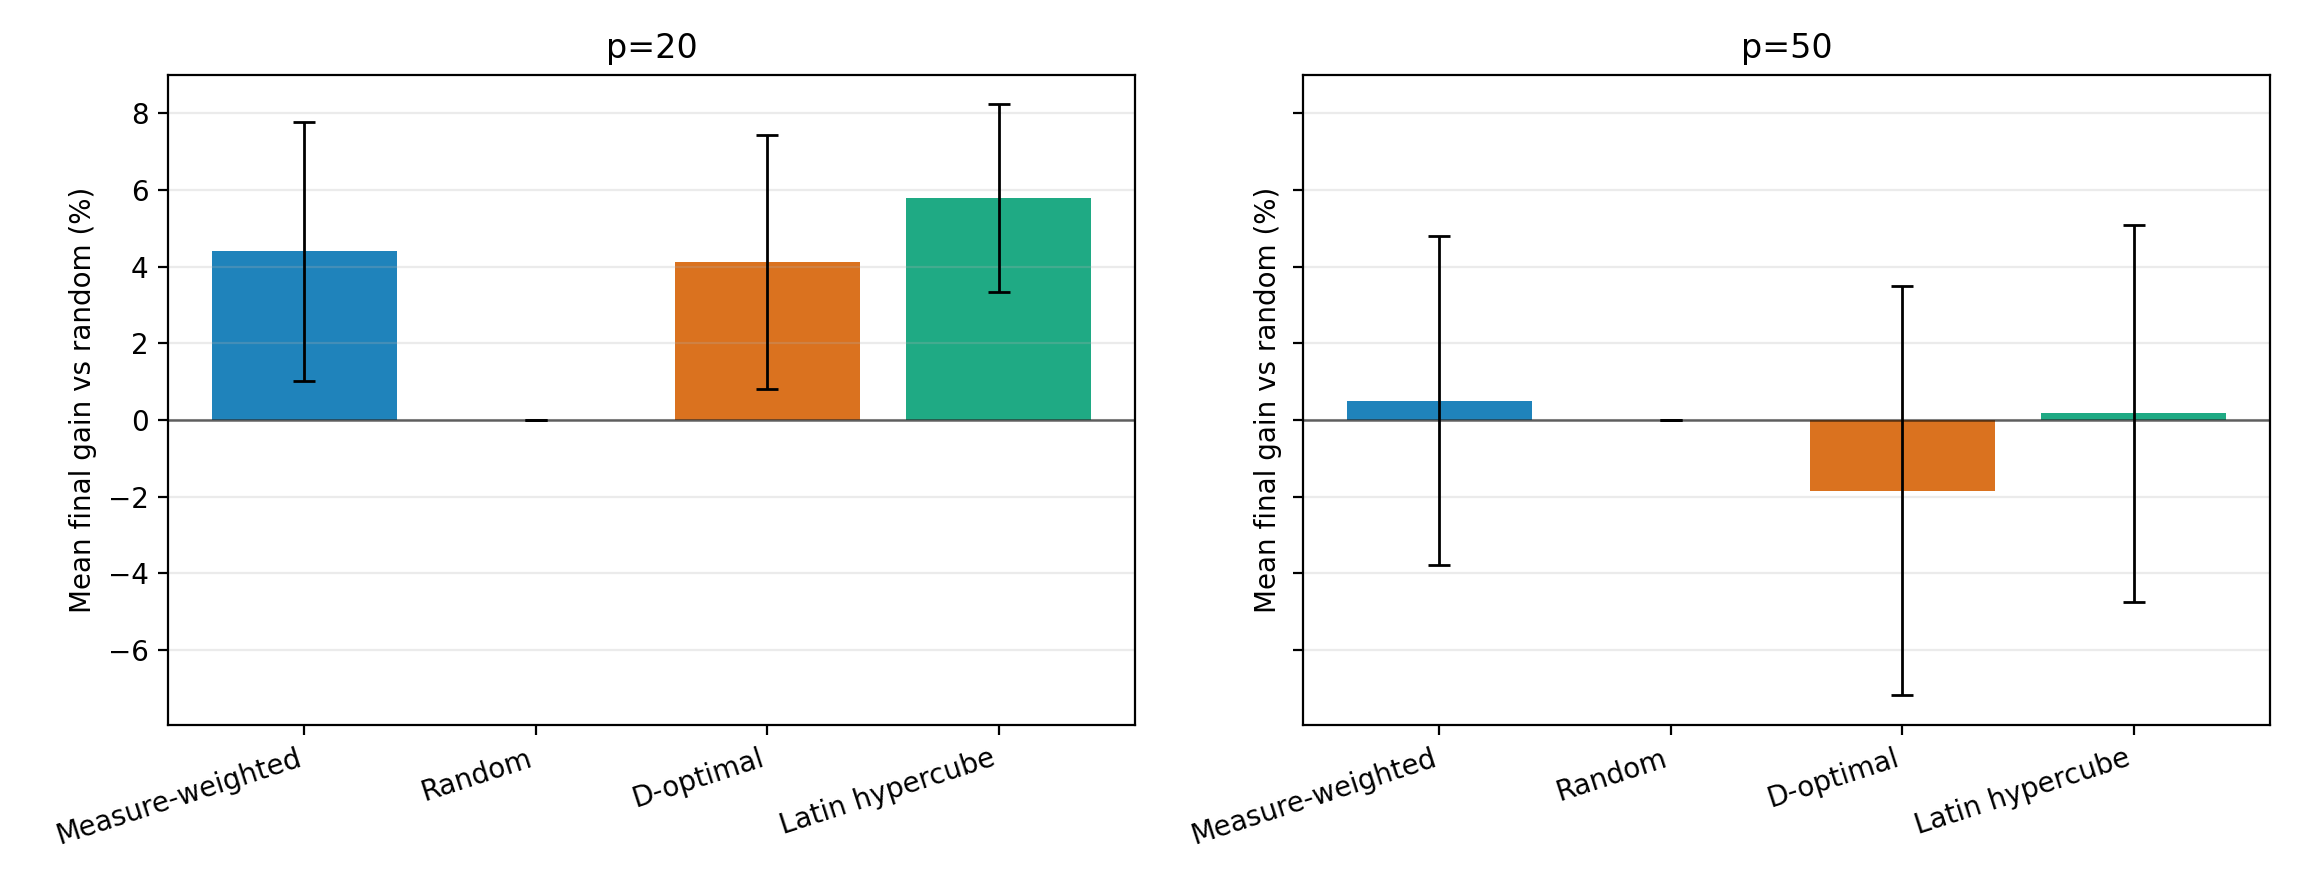
\includegraphics[width=0.92\textwidth]{figures/measure_weighted/measure_weighted_grand_gain_by_p.png}
\caption{不同维度下各策略相对随机采样的最终提升}
\end{figure}

\begin{figure}[htbp]
\centering
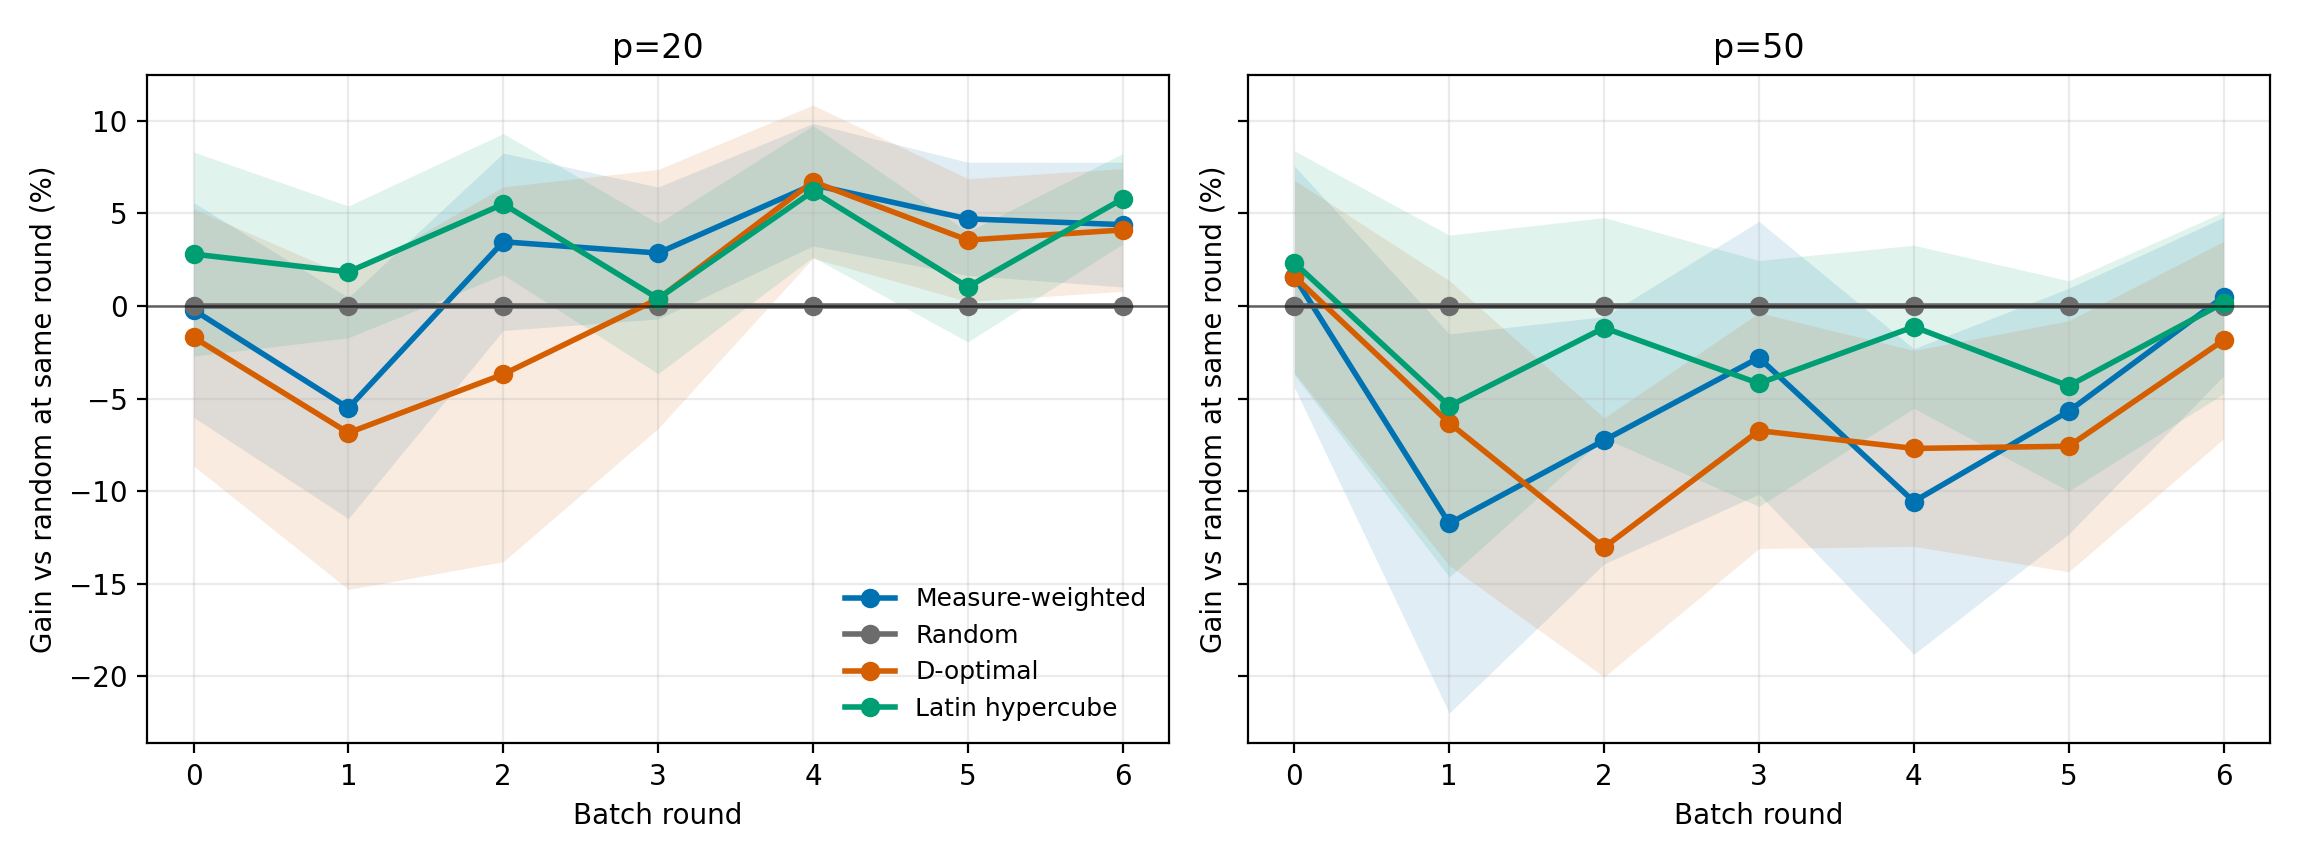
\includegraphics[width=0.92\textwidth]{figures/measure_weighted/measure_weighted_grand_learning_gain.png}
\caption{多轮 batch 更新中的相对随机提升曲线}
\end{figure}

\subsection{4. 分数据集结果}

Measure-weighted 在 p=20 的多数结构上为正提升，在 p=50 中能明显缓解全 D-optimal 的负迁移，尤其在 high-frequency 中将全 D-optimal 的大幅损失压回接近随机水平，在 local interior 中则取得最强结果。

\begin{longtable}{p{0.190\textwidth}p{0.190\textwidth}p{0.190\textwidth}p{0.190\textwidth}p{0.190\textwidth}}
\toprule
p & 数据集 & Measure-weighted MSE & 相对随机提升 & 正提升率 \\
\midrule
\endfirsthead
\toprule
p & 数据集 & Measure-weighted MSE & 相对随机提升 & 正提升率 \\
\midrule
\endhead
20 & 高频非多项式 & 0.010106 & -9.52\% & 40.0\% \\
20 & 局部内部结构 & 0.003893 & 5.82\% & 80.0\% \\
20 & 二次多项式 & 0.007036 & 8.24\% & 90.0\% \\
20 & 平滑非线性 & 0.002244 & 8.96\% & 90.0\% \\
20 & 强非线性 & 0.001685 & 8.48\% & 60.0\% \\
50 & 高频非多项式 & 0.022579 & 0.24\% & 60.0\% \\
50 & 局部内部结构 & 0.008042 & 13.55\% & 80.0\% \\
50 & 二次多项式 & 0.049157 & -8.05\% & 30.0\% \\
50 & 平滑非线性 & 0.010861 & -2.91\% & 30.0\% \\
50 & 强非线性 & 0.005076 & -0.33\% & 70.0\% \\
\bottomrule
\end{longtable}

\begin{figure}[htbp]
\centering
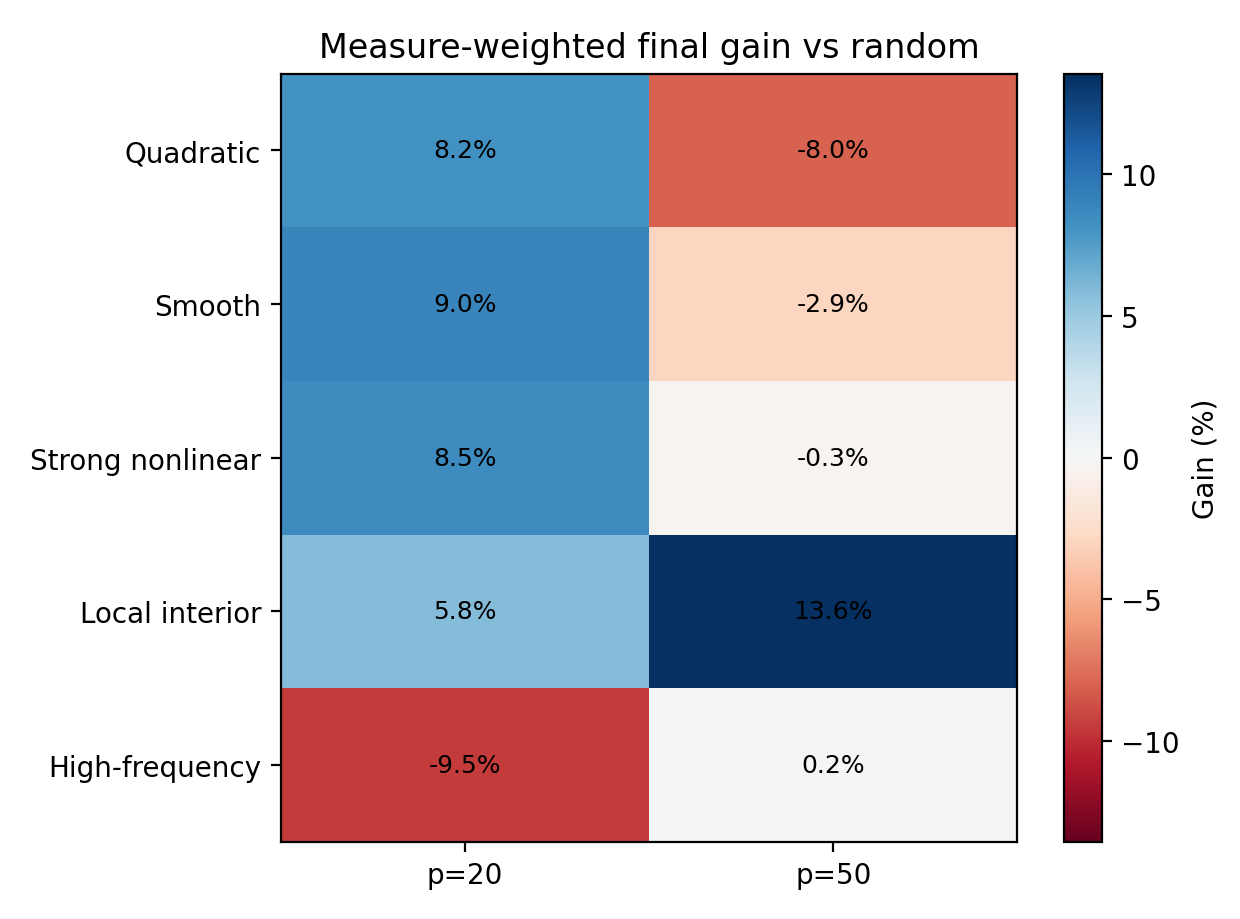
\includegraphics[width=0.92\textwidth]{figures/measure_weighted/measure_weighted_grand_case_gain_heatmap.png}
\caption{Measure-weighted 在各数据集和维度下的相对随机提升}
\end{figure}

\subsection{5. 权重校准与测度解释}

权重热图显示，采样比例不是按数据集标签硬编码，而是由每个 pilot run 的距离决定。p=20 中 high-frequency 被压到低 D-optimal 比例；p=50 中某些情形的权重明显下降，说明维度升高后 PR/TYPR 近似性变弱时，策略会自动更保守。

\begin{longtable}{p{0.190\textwidth}p{0.190\textwidth}p{0.190\textwidth}p{0.190\textwidth}p{0.190\textwidth}}
\toprule
p & 数据集 & FPR 距离均值 & TYPR 距离均值 & D-optimal 比例均值 \\
\midrule
\endfirsthead
\toprule
p & 数据集 & FPR 距离均值 & TYPR 距离均值 & D-optimal 比例均值 \\
\midrule
\endhead
20 & 高频非多项式 & 0.22958 & 0.94323 & 0.323 \\
20 & 局部内部结构 & 0.08290 & 0.90947 & 0.551 \\
20 & 二次多项式 & 0.04888 & 0.92314 & 0.579 \\
20 & 平滑非线性 & 0.01406 & 0.78233 & 0.779 \\
20 & 强非线性 & 0.01903 & 0.80521 & 0.749 \\
50 & 高频非多项式 & 0.01115 & 0.87244 & 0.377 \\
50 & 局部内部结构 & 0.00287 & 0.69602 & 0.545 \\
50 & 二次多项式 & 0.00381 & 0.67319 & 0.578 \\
50 & 平滑非线性 & 0.00507 & 0.53331 & 0.694 \\
50 & 强非线性 & 0.00797 & 0.42922 & 0.815 \\
\bottomrule
\end{longtable}

\begin{figure}[htbp]
\centering
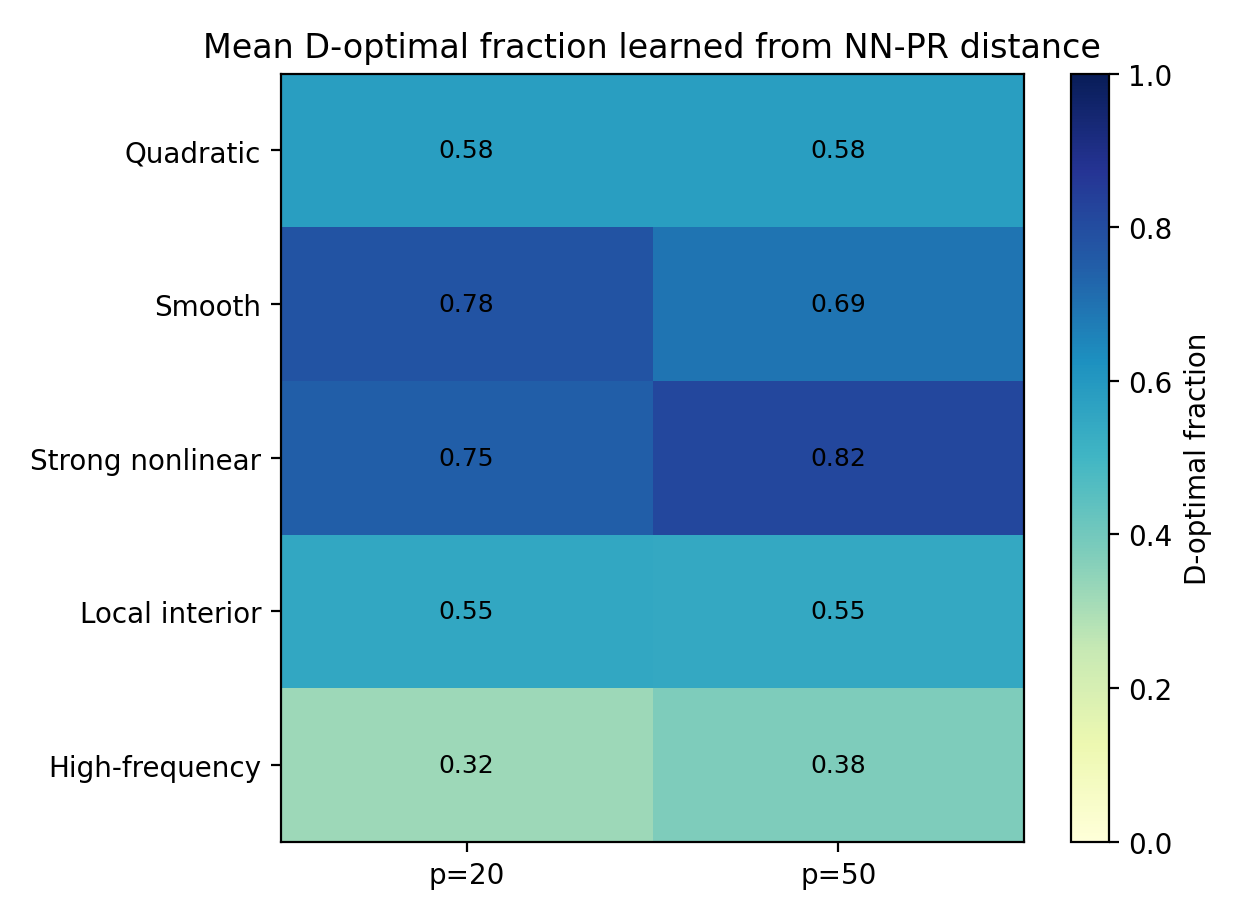
\includegraphics[width=0.92\textwidth]{figures/measure_weighted/measure_weighted_grand_weight_heatmap.png}
\caption{由 NN-PR/TYPR 距离学习到的 D-optimal 平均比例}
\end{figure}

\subsection{6. 敏感性与边界条件}

\begin{longtable}{p{0.280\textwidth}}
\toprule
重要修正 早先使用 min(d\_FPR, d\_TYPR) 时，p=50 的 Measure-weighted 相对随机为 -2.821\%；改用 mean(d\_FPR, d\_TYPR) 后提高到 +0.501\%，并超过全 D-optimal 的 -1.846\%。这说明高维下需要更保守的距离组合规则。 \\
\midrule
\endfirsthead
\toprule
重要修正 早先使用 min(d\_FPR, d\_TYPR) 时，p=50 的 Measure-weighted 相对随机为 -2.821\%；改用 mean(d\_FPR, d\_TYPR) 后提高到 +0.501\%，并超过全 D-optimal 的 -1.846\%。这说明高维下需要更保守的距离组合规则。 \\
\midrule
\endhead
\bottomrule
\end{longtable}

\begin{itemize}
\item 优势：该测度能把采样策略从固定规则变成数据驱动规则，尤其能识别 D-optimal 可能负迁移的场景。
\end{itemize}

\begin{itemize}
\item 限制：Latin hypercube 在某些高频或全局覆盖需求强的场景仍然更稳定；当前策略只在随机和 D-optimal 之间混合，尚未把 Latin 作为可选动作。
\end{itemize}

\begin{itemize}
\item 后续改进：可把 D-optimal 下限从 30\% 降到 10\% 或引入三路混合（random / D-optimal / Latin），让远距离场景更接近纯探索。
\end{itemize}

\section{高维迭代 D-optimal 实验：数据与数据分析}
\noindent\textbf{来源文件：}reports/zh/大报告\_中文\_完整版\_论文级高维迭代更新版.docx

\subsection{实验流程}

\begin{itemize}
\item 先生成原始高维数据集，并按 75/25 划分为训练池和评估集。
\end{itemize}

\begin{itemize}
\item 在训练池上训练 NN oracle，将该 NN 视为新的目标模型。
\end{itemize}

\begin{itemize}
\item 从训练池中均匀抽取初始设计集，估计 NN 与 FullPR surrogate 的 pilot 距离。
\end{itemize}

\begin{itemize}
\item 每一轮基于当前已经升级后的设计集计算 D-optimal leverage，选择下一批样本加入设计集。
\end{itemize}

\begin{itemize}
\item 每轮重新拟合 FullPR surrogate，并与同预算随机升级的中位数表现比较。
\end{itemize}

\subsection{实验矩阵与计算量}

\begin{longtable}{p{0.280\textwidth}p{0.280\textwidth}}
\toprule
项目 & 设置 \\
\midrule
\endfirsthead
\toprule
项目 & 设置 \\
\midrule
\endhead
原始数据集大小 & 10000 \\
输入维度 & 20, 50 \\
数据场景 & quadratic, smooth, strong nonlinear \\
初始 uniform 比例 & 0.05, 0.1 \\
迭代轮数 & 5；每轮增加 500 个样本 \\
随机基准 & 每个迭代点重复 10 次 \\
设备 & CPU 与 NVIDIA GeForce RTX 4070 Ti SUPER \\
FullPR 特征 & degree=2, include\_special=True \\
\bottomrule
\end{longtable}

\subsection{主要结果}

\begin{figure}[htbp]
\centering
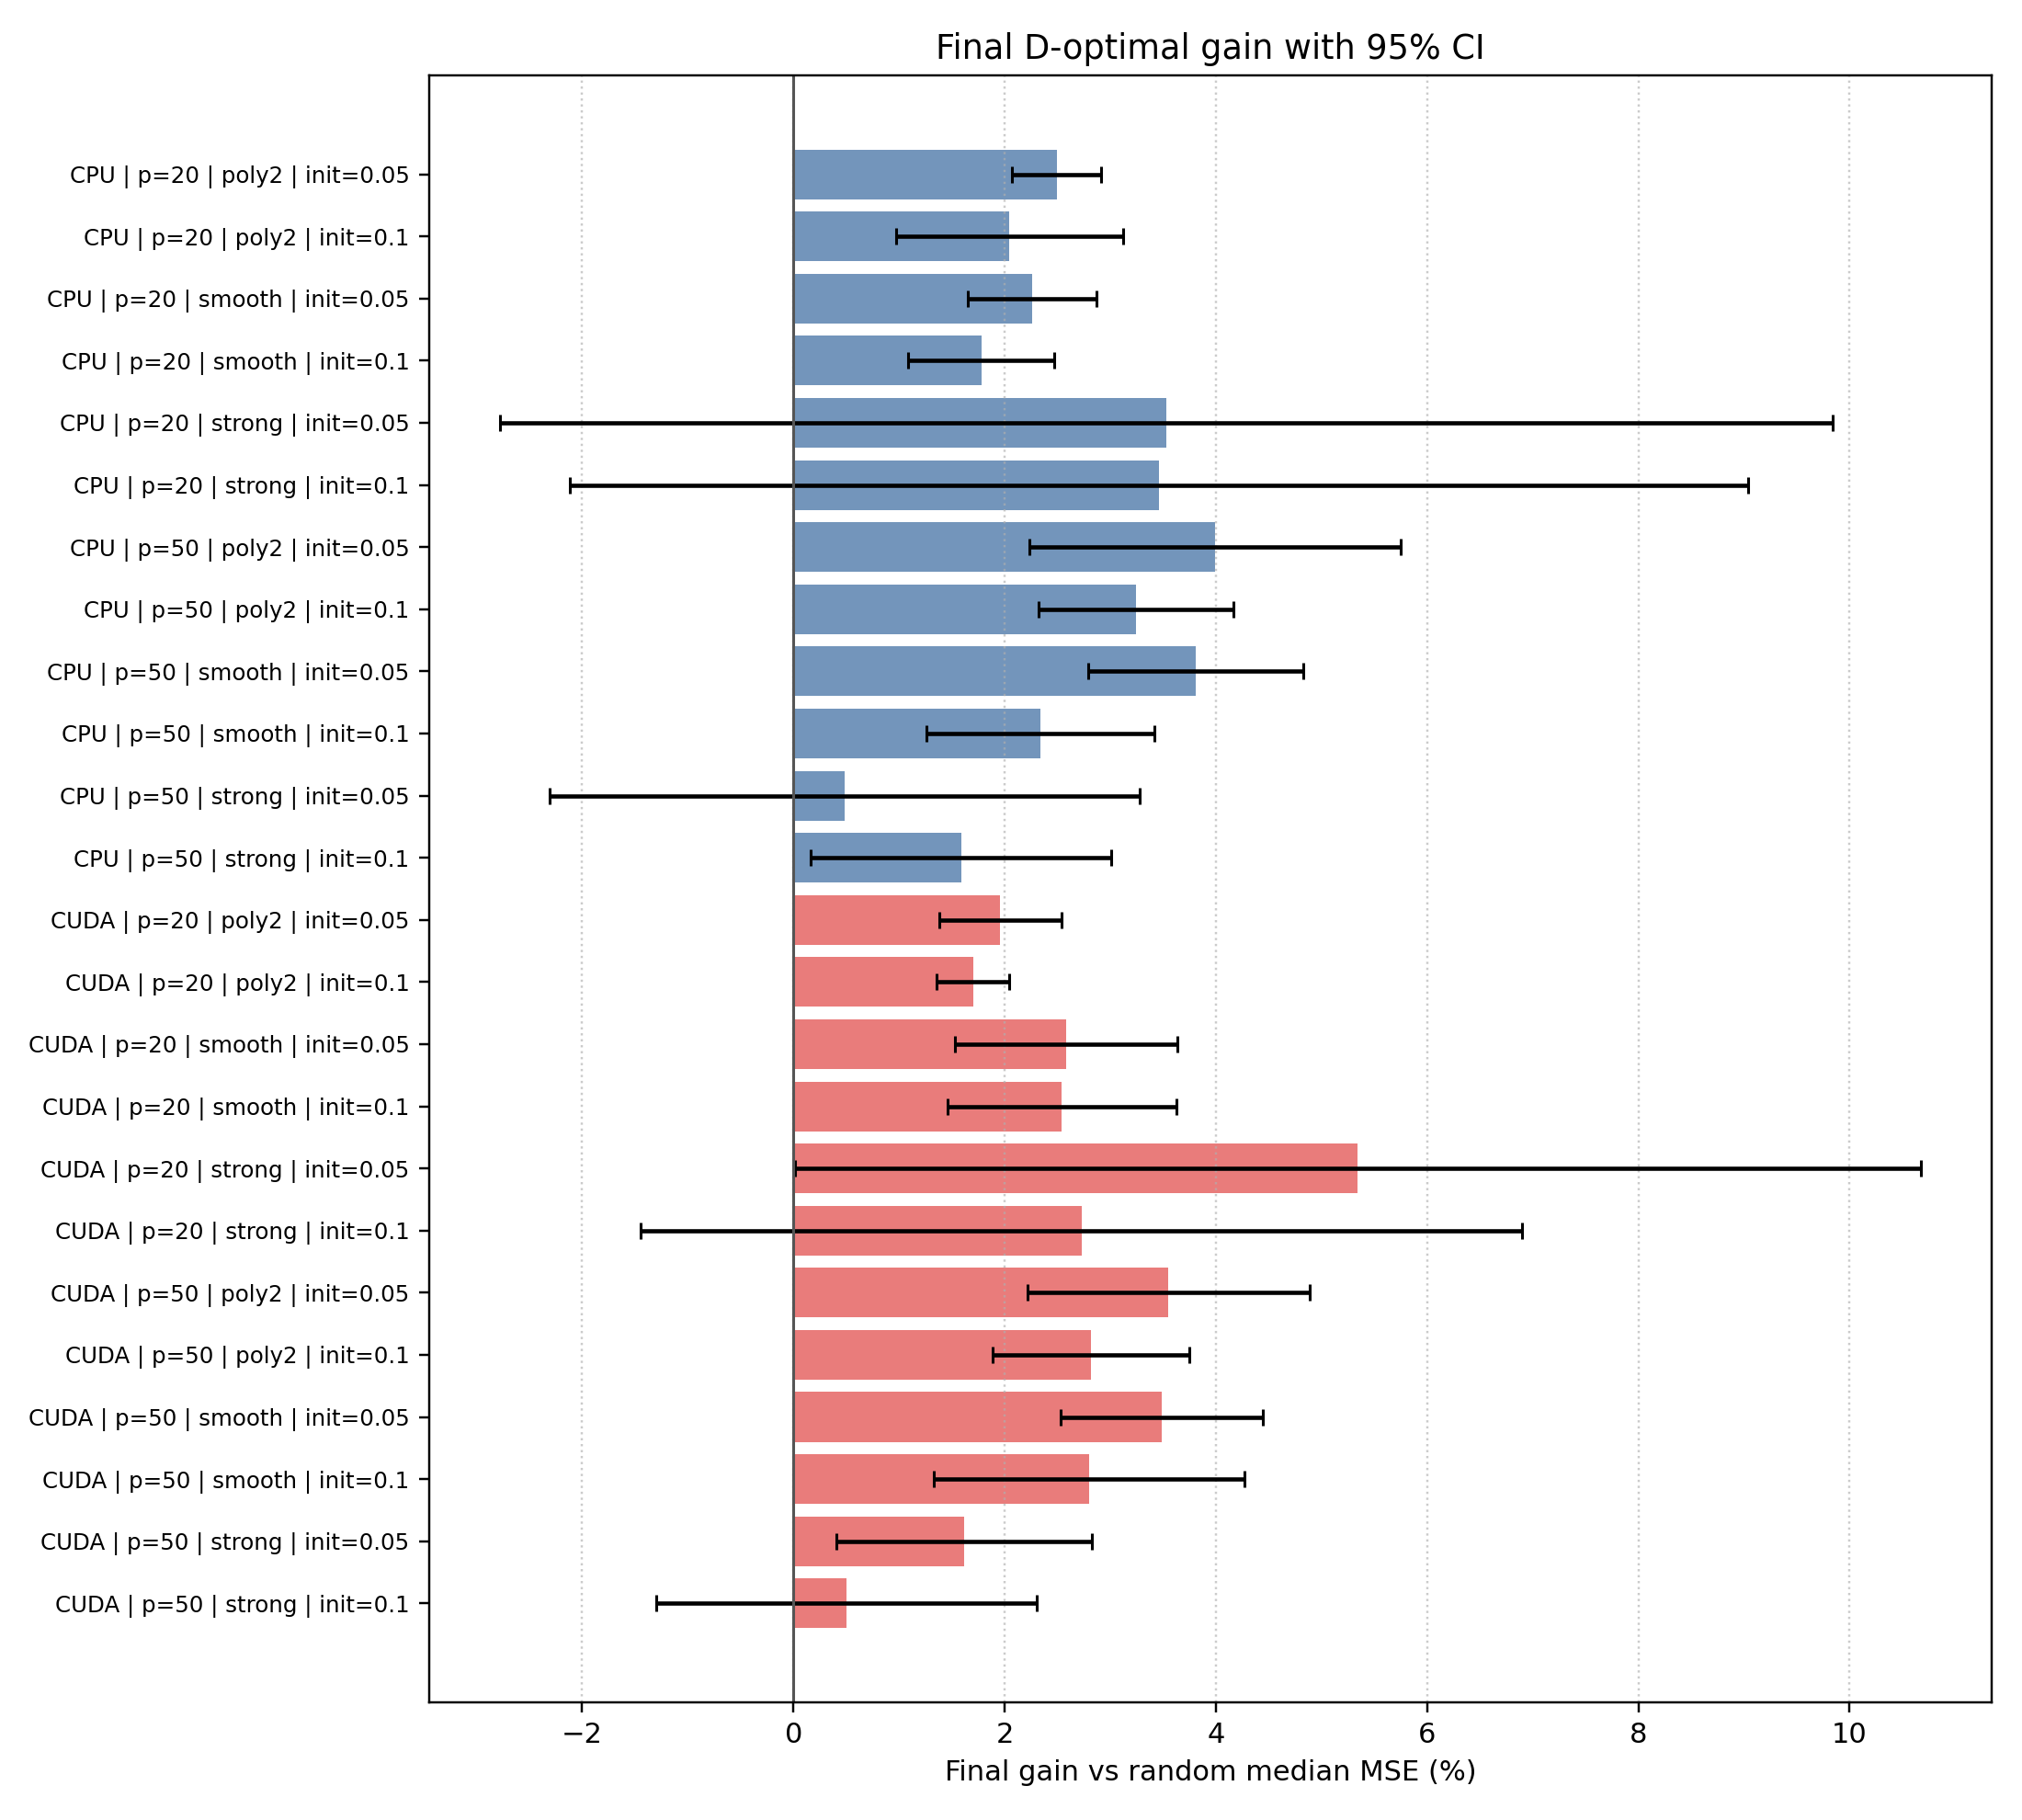
\includegraphics[width=0.92\textwidth]{figures/highdim_iter/paper_highdim_iter_dopt_final_gain_ci.png}
\caption{最后一轮 D-optimal 相对随机升级的 mean gain +/- 95\% CI。}
\end{figure}

\subsubsection{最后一轮分组统计}

表 1 和表 2 汇总最后一轮结果。gain 为正表示 D-optimal surrogate 的 MSE 低于同预算随机升级中位数。

\begin{longtable}{p{0.158\textwidth}p{0.158\textwidth}p{0.158\textwidth}p{0.158\textwidth}p{0.158\textwidth}p{0.158\textwidth}}
\toprule
Case & p & Init & Reps & Gain mean +/-95\%CI & Positive \\
\midrule
\endfirsthead
\toprule
Case & p & Init & Reps & Gain mean +/-95\%CI & Positive \\
\midrule
\endhead
poly2 & 20 & 0.05 & 6 & 2.49\% +/- 0.43\% & 100.0\% \\
poly2 & 20 & 0.1 & 6 & 2.04\% +/- 1.08\% & 83.3\% \\
smooth & 20 & 0.05 & 6 & 2.26\% +/- 0.61\% & 100.0\% \\
smooth & 20 & 0.1 & 6 & 1.78\% +/- 0.69\% & 100.0\% \\
strong & 20 & 0.05 & 6 & 3.53\% +/- 6.31\% & 66.7\% \\
strong & 20 & 0.1 & 6 & 3.46\% +/- 5.58\% & 66.7\% \\
poly2 & 50 & 0.05 & 6 & 3.99\% +/- 1.76\% & 100.0\% \\
poly2 & 50 & 0.1 & 6 & 3.24\% +/- 0.92\% & 100.0\% \\
smooth & 50 & 0.05 & 6 & 3.81\% +/- 1.02\% & 100.0\% \\
smooth & 50 & 0.1 & 6 & 2.34\% +/- 1.08\% & 100.0\% \\
strong & 50 & 0.05 & 6 & 0.48\% +/- 2.79\% & 66.7\% \\
strong & 50 & 0.1 & 6 & 1.59\% +/- 1.42\% & 66.7\% \\
\bottomrule
\end{longtable}

\begin{longtable}{p{0.158\textwidth}p{0.158\textwidth}p{0.158\textwidth}p{0.158\textwidth}p{0.158\textwidth}p{0.158\textwidth}}
\toprule
Case & p & Init & Reps & Gain mean +/-95\%CI & Positive \\
\midrule
\endfirsthead
\toprule
Case & p & Init & Reps & Gain mean +/-95\%CI & Positive \\
\midrule
\endhead
poly2 & 20 & 0.05 & 6 & 1.96\% +/- 0.58\% & 100.0\% \\
poly2 & 20 & 0.1 & 6 & 1.70\% +/- 0.34\% & 100.0\% \\
smooth & 20 & 0.05 & 6 & 2.58\% +/- 1.05\% & 100.0\% \\
smooth & 20 & 0.1 & 6 & 2.54\% +/- 1.08\% & 100.0\% \\
strong & 20 & 0.05 & 6 & 5.35\% +/- 5.33\% & 83.3\% \\
strong & 20 & 0.1 & 6 & 2.73\% +/- 4.17\% & 66.7\% \\
poly2 & 50 & 0.05 & 6 & 3.55\% +/- 1.34\% & 100.0\% \\
poly2 & 50 & 0.1 & 6 & 2.82\% +/- 0.93\% & 100.0\% \\
smooth & 50 & 0.05 & 6 & 3.49\% +/- 0.96\% & 100.0\% \\
smooth & 50 & 0.1 & 6 & 2.80\% +/- 1.47\% & 83.3\% \\
strong & 50 & 0.05 & 6 & 1.62\% +/- 1.21\% & 83.3\% \\
strong & 50 & 0.1 & 6 & 0.50\% +/- 1.80\% & 66.7\% \\
\bottomrule
\end{longtable}

\subsection{迭代曲线}

\begin{figure}[htbp]
\centering
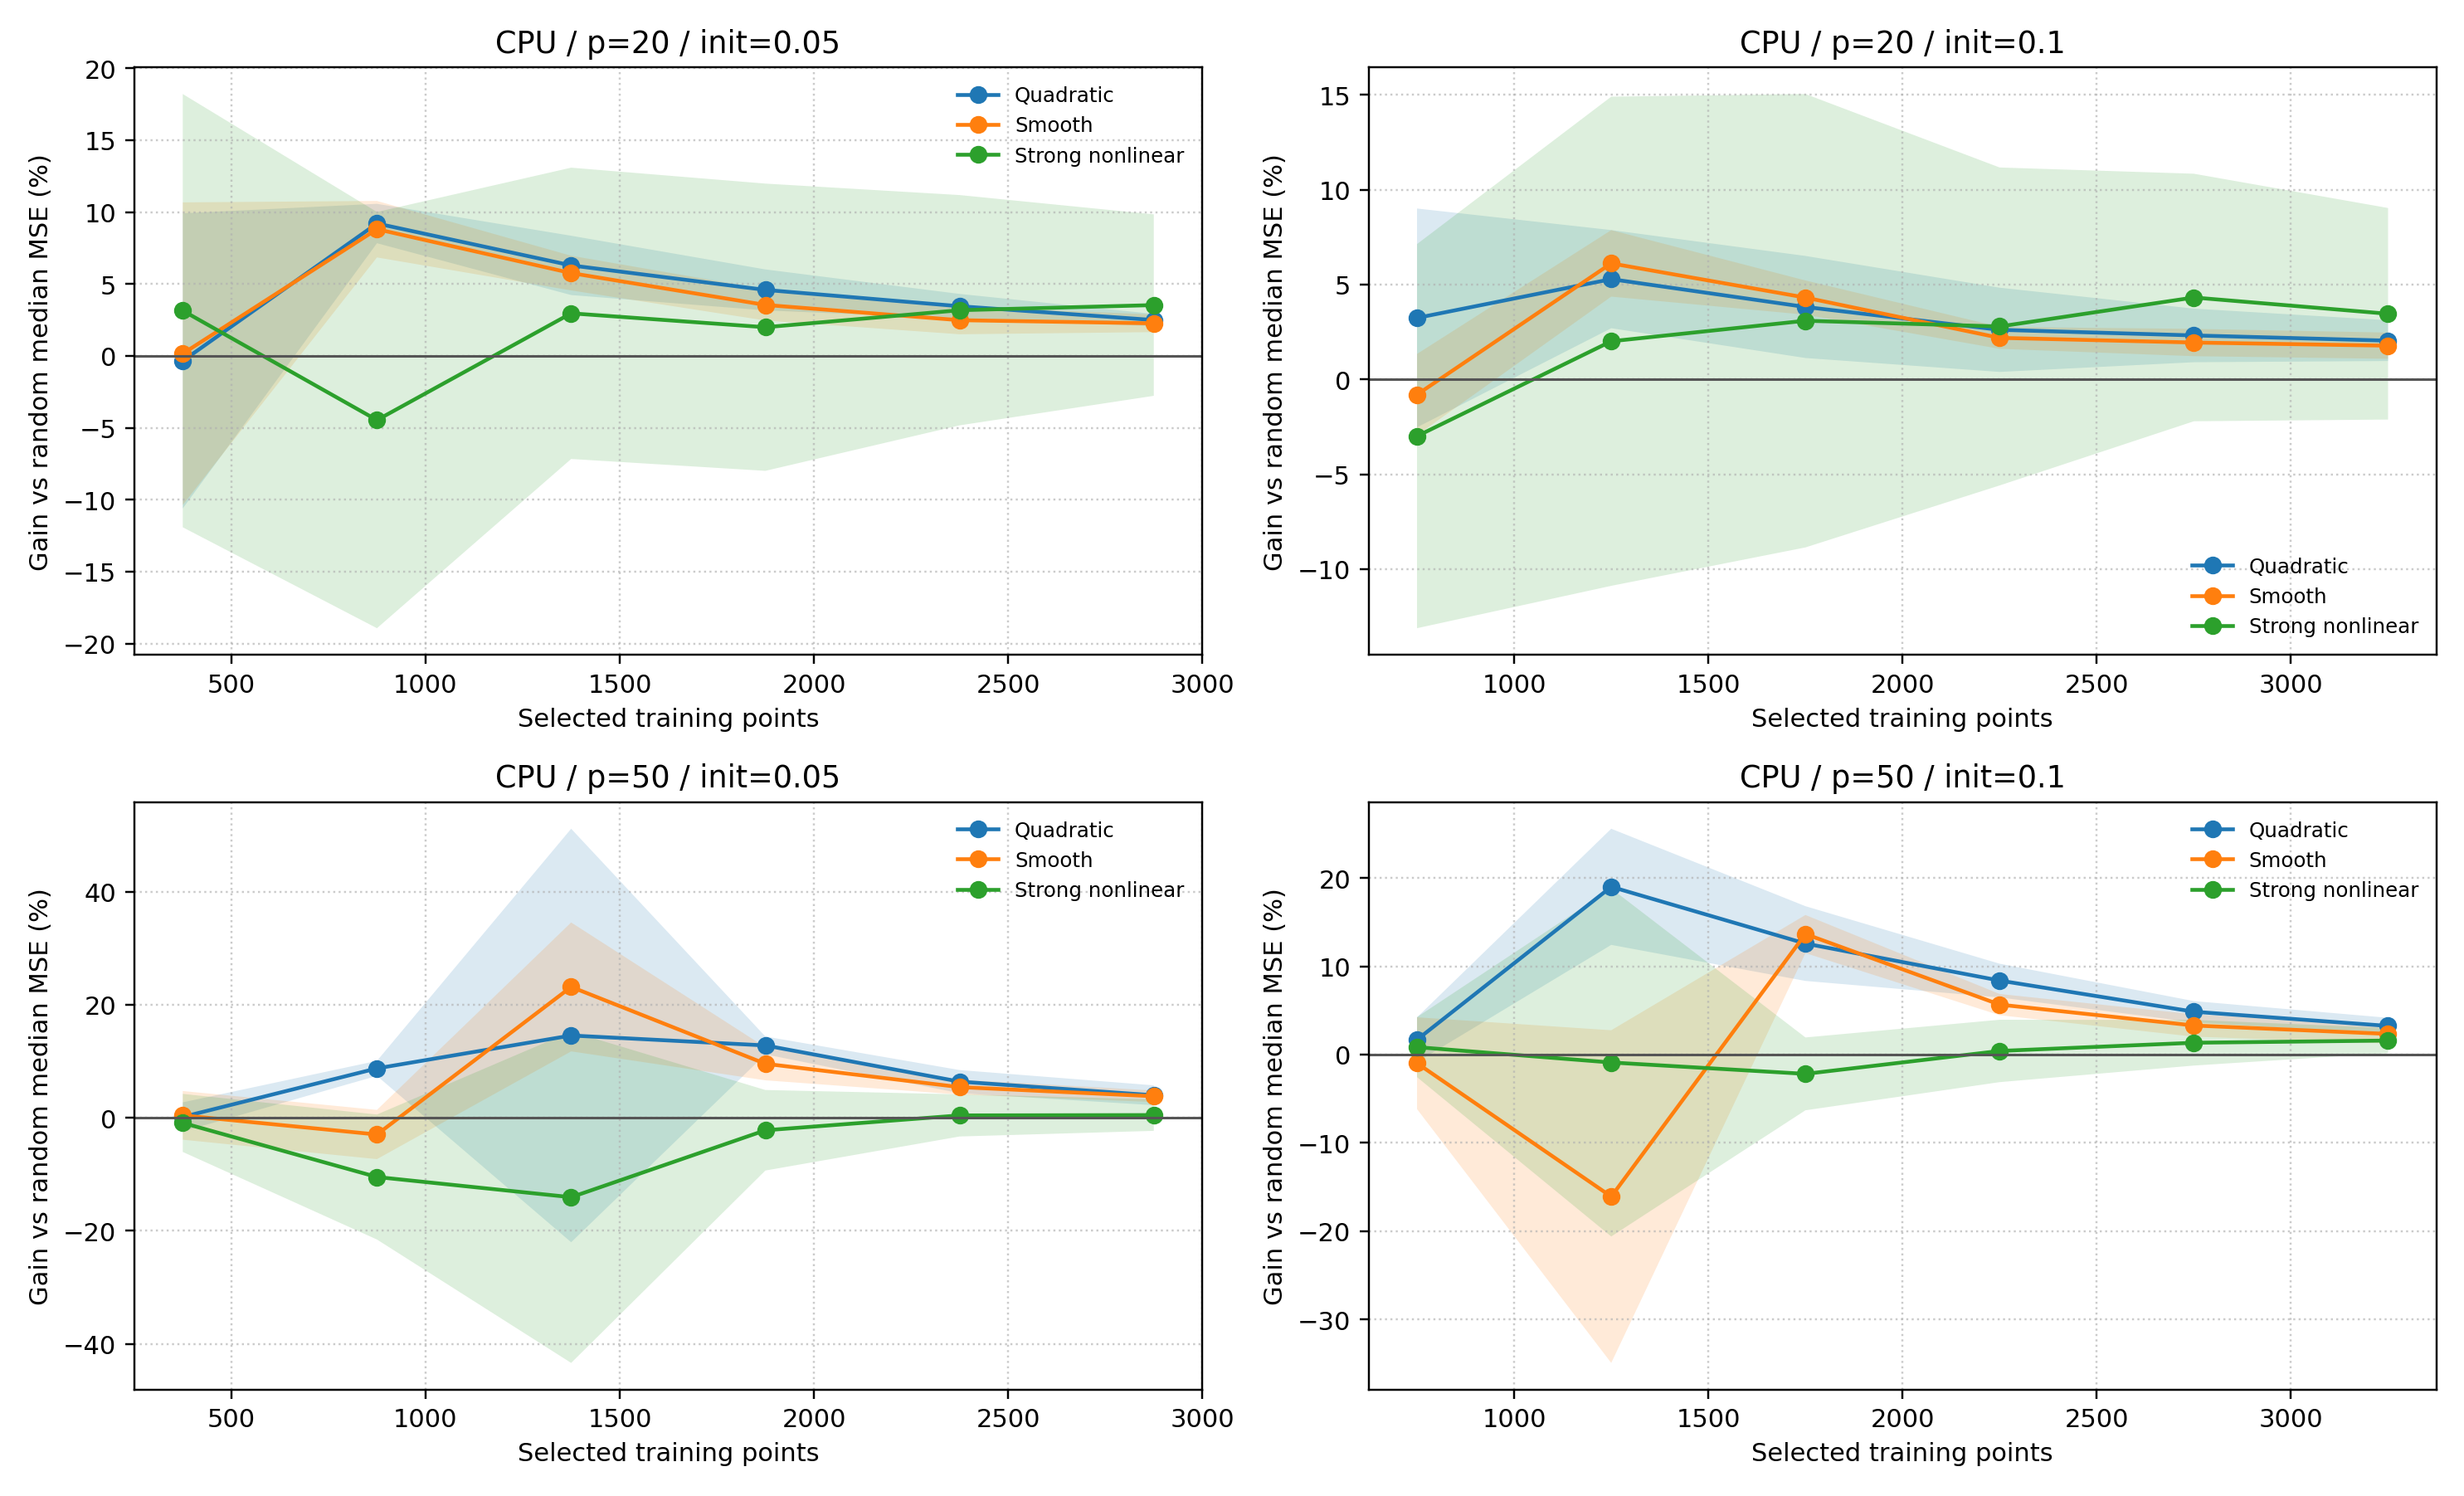
\includegraphics[width=0.92\textwidth]{figures/highdim_iter/paper_highdim_iter_dopt_cpu_gain_mean_ci.png}
\caption{CPU 实验中 D-optimal 相对随机升级的 gain 均值曲线与 95\% CI。}
\end{figure}

\begin{figure}[htbp]
\centering
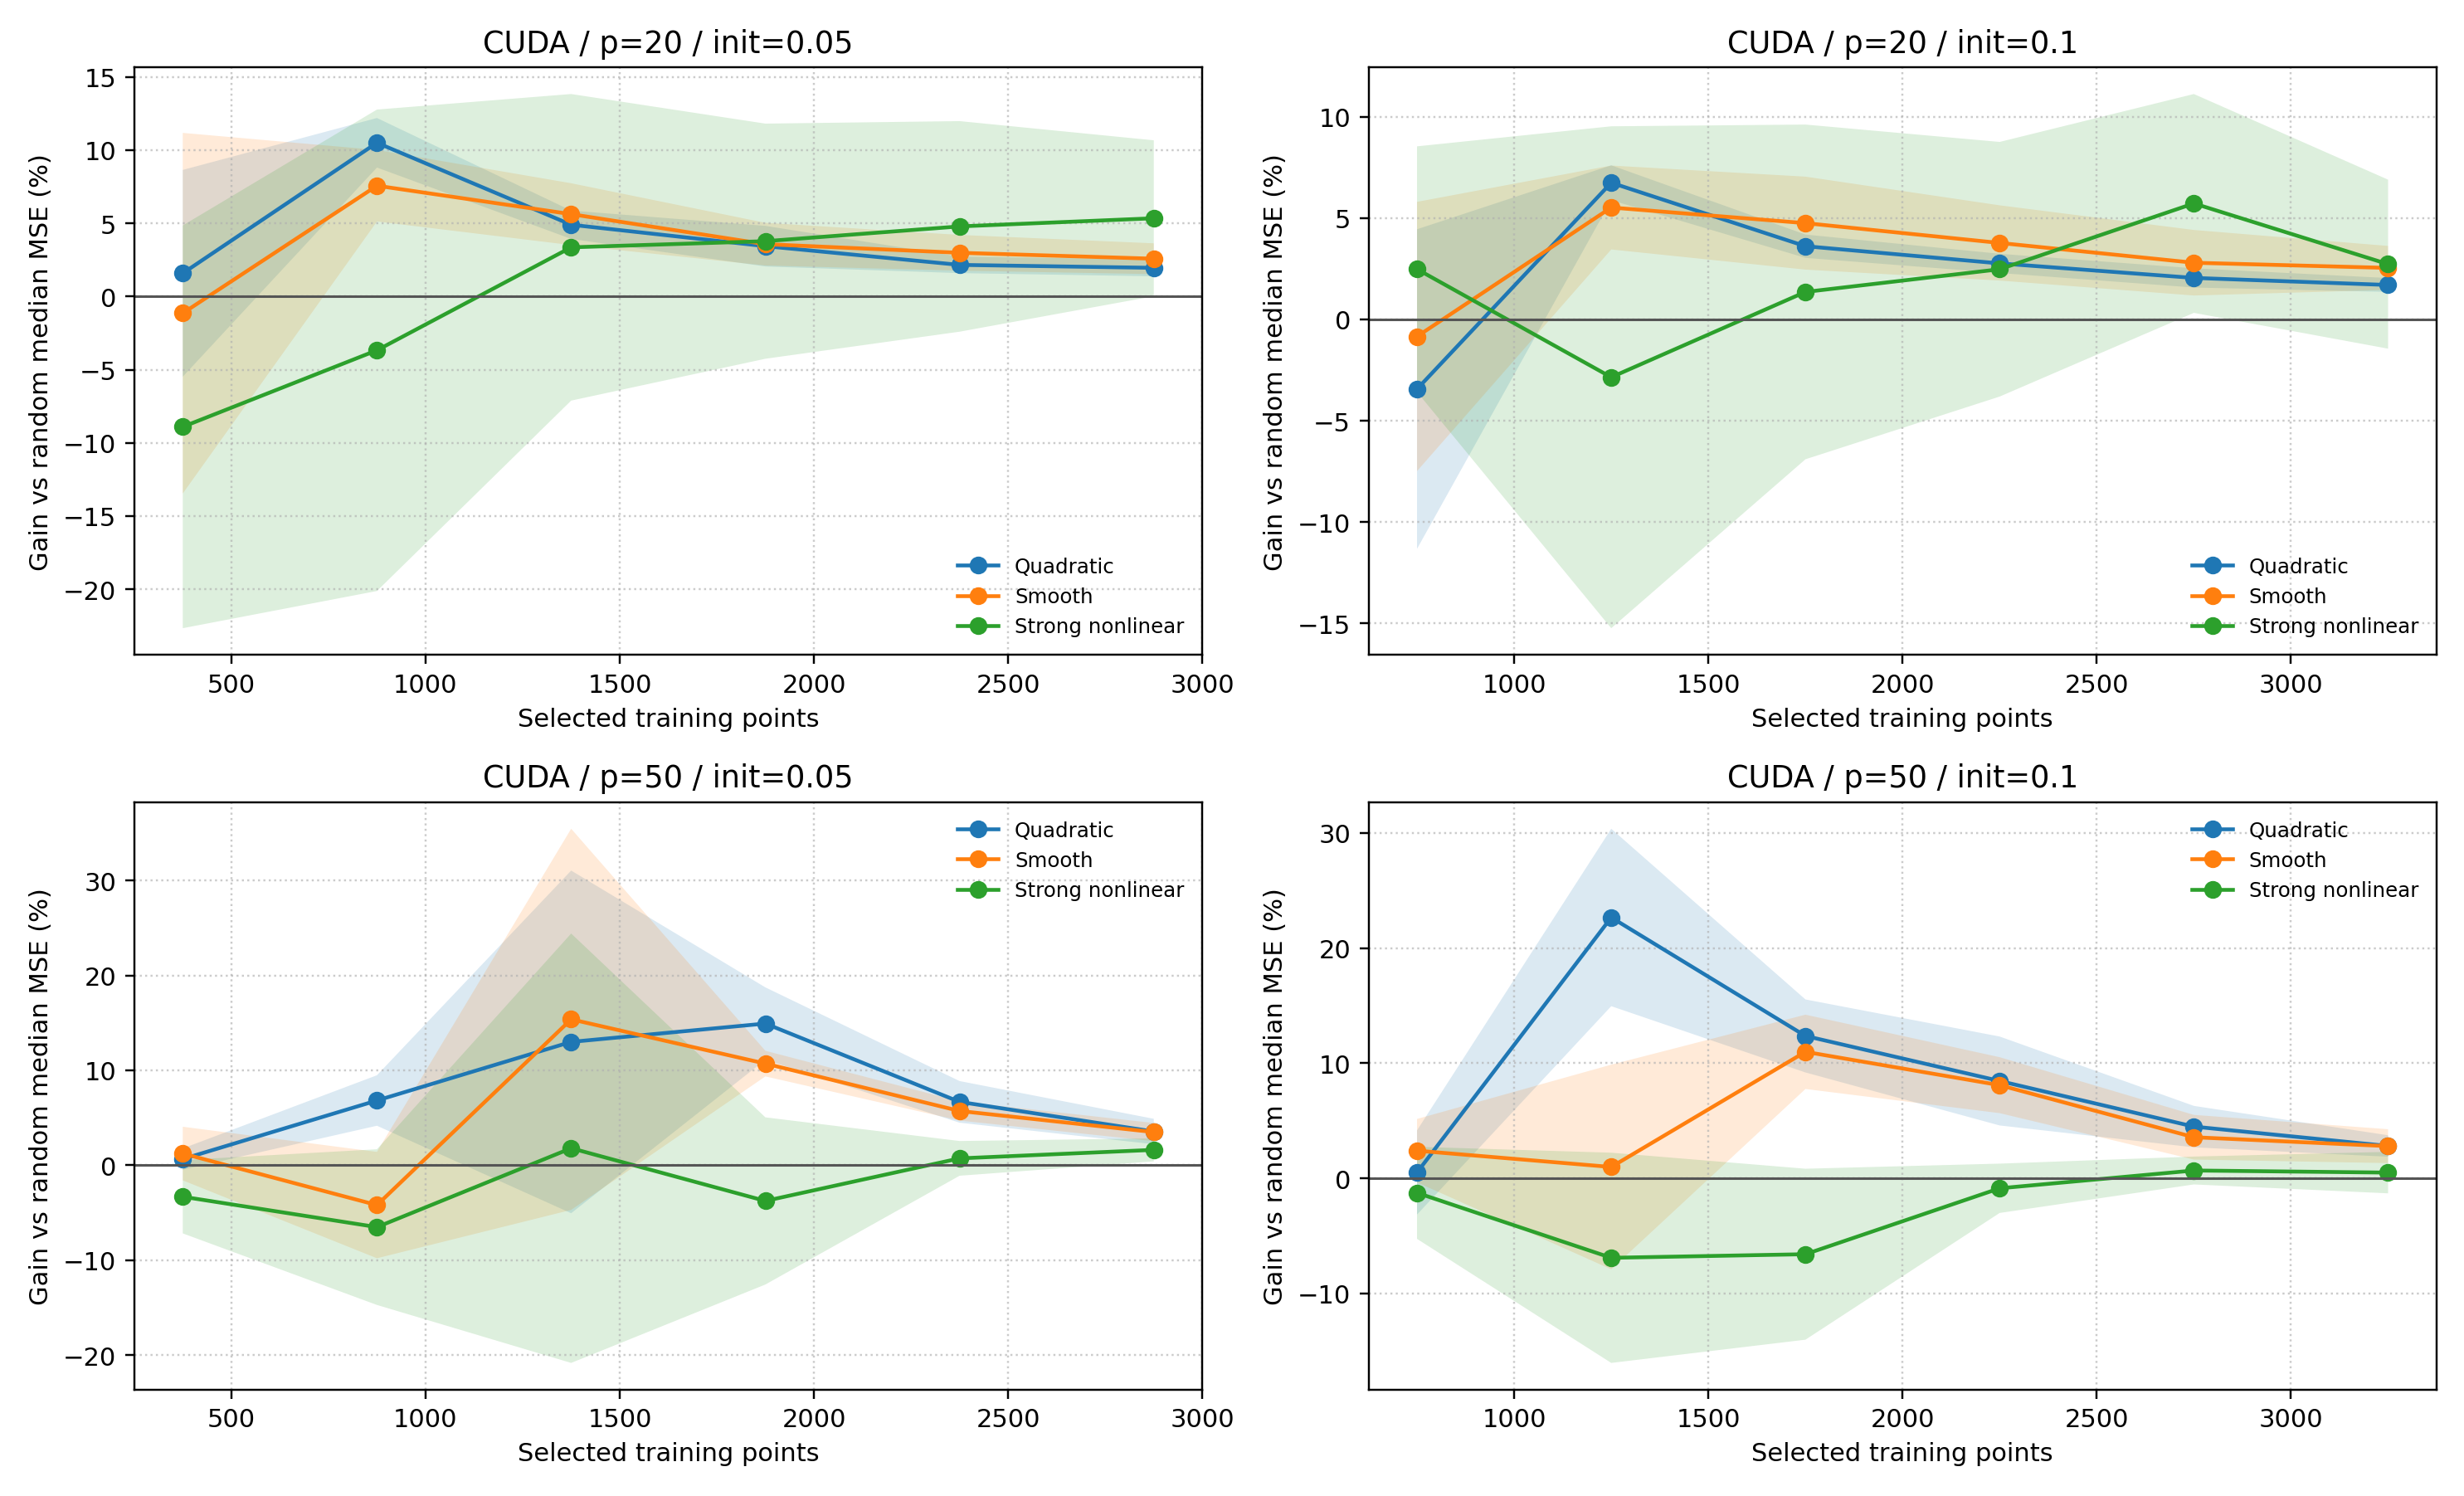
\includegraphics[width=0.92\textwidth]{figures/highdim_iter/paper_highdim_iter_dopt_cuda_gain_mean_ci.png}
\caption{CUDA 实验中 D-optimal 相对随机升级的 gain 均值曲线与 95\% CI。}
\end{figure}

\begin{figure}[htbp]
\centering
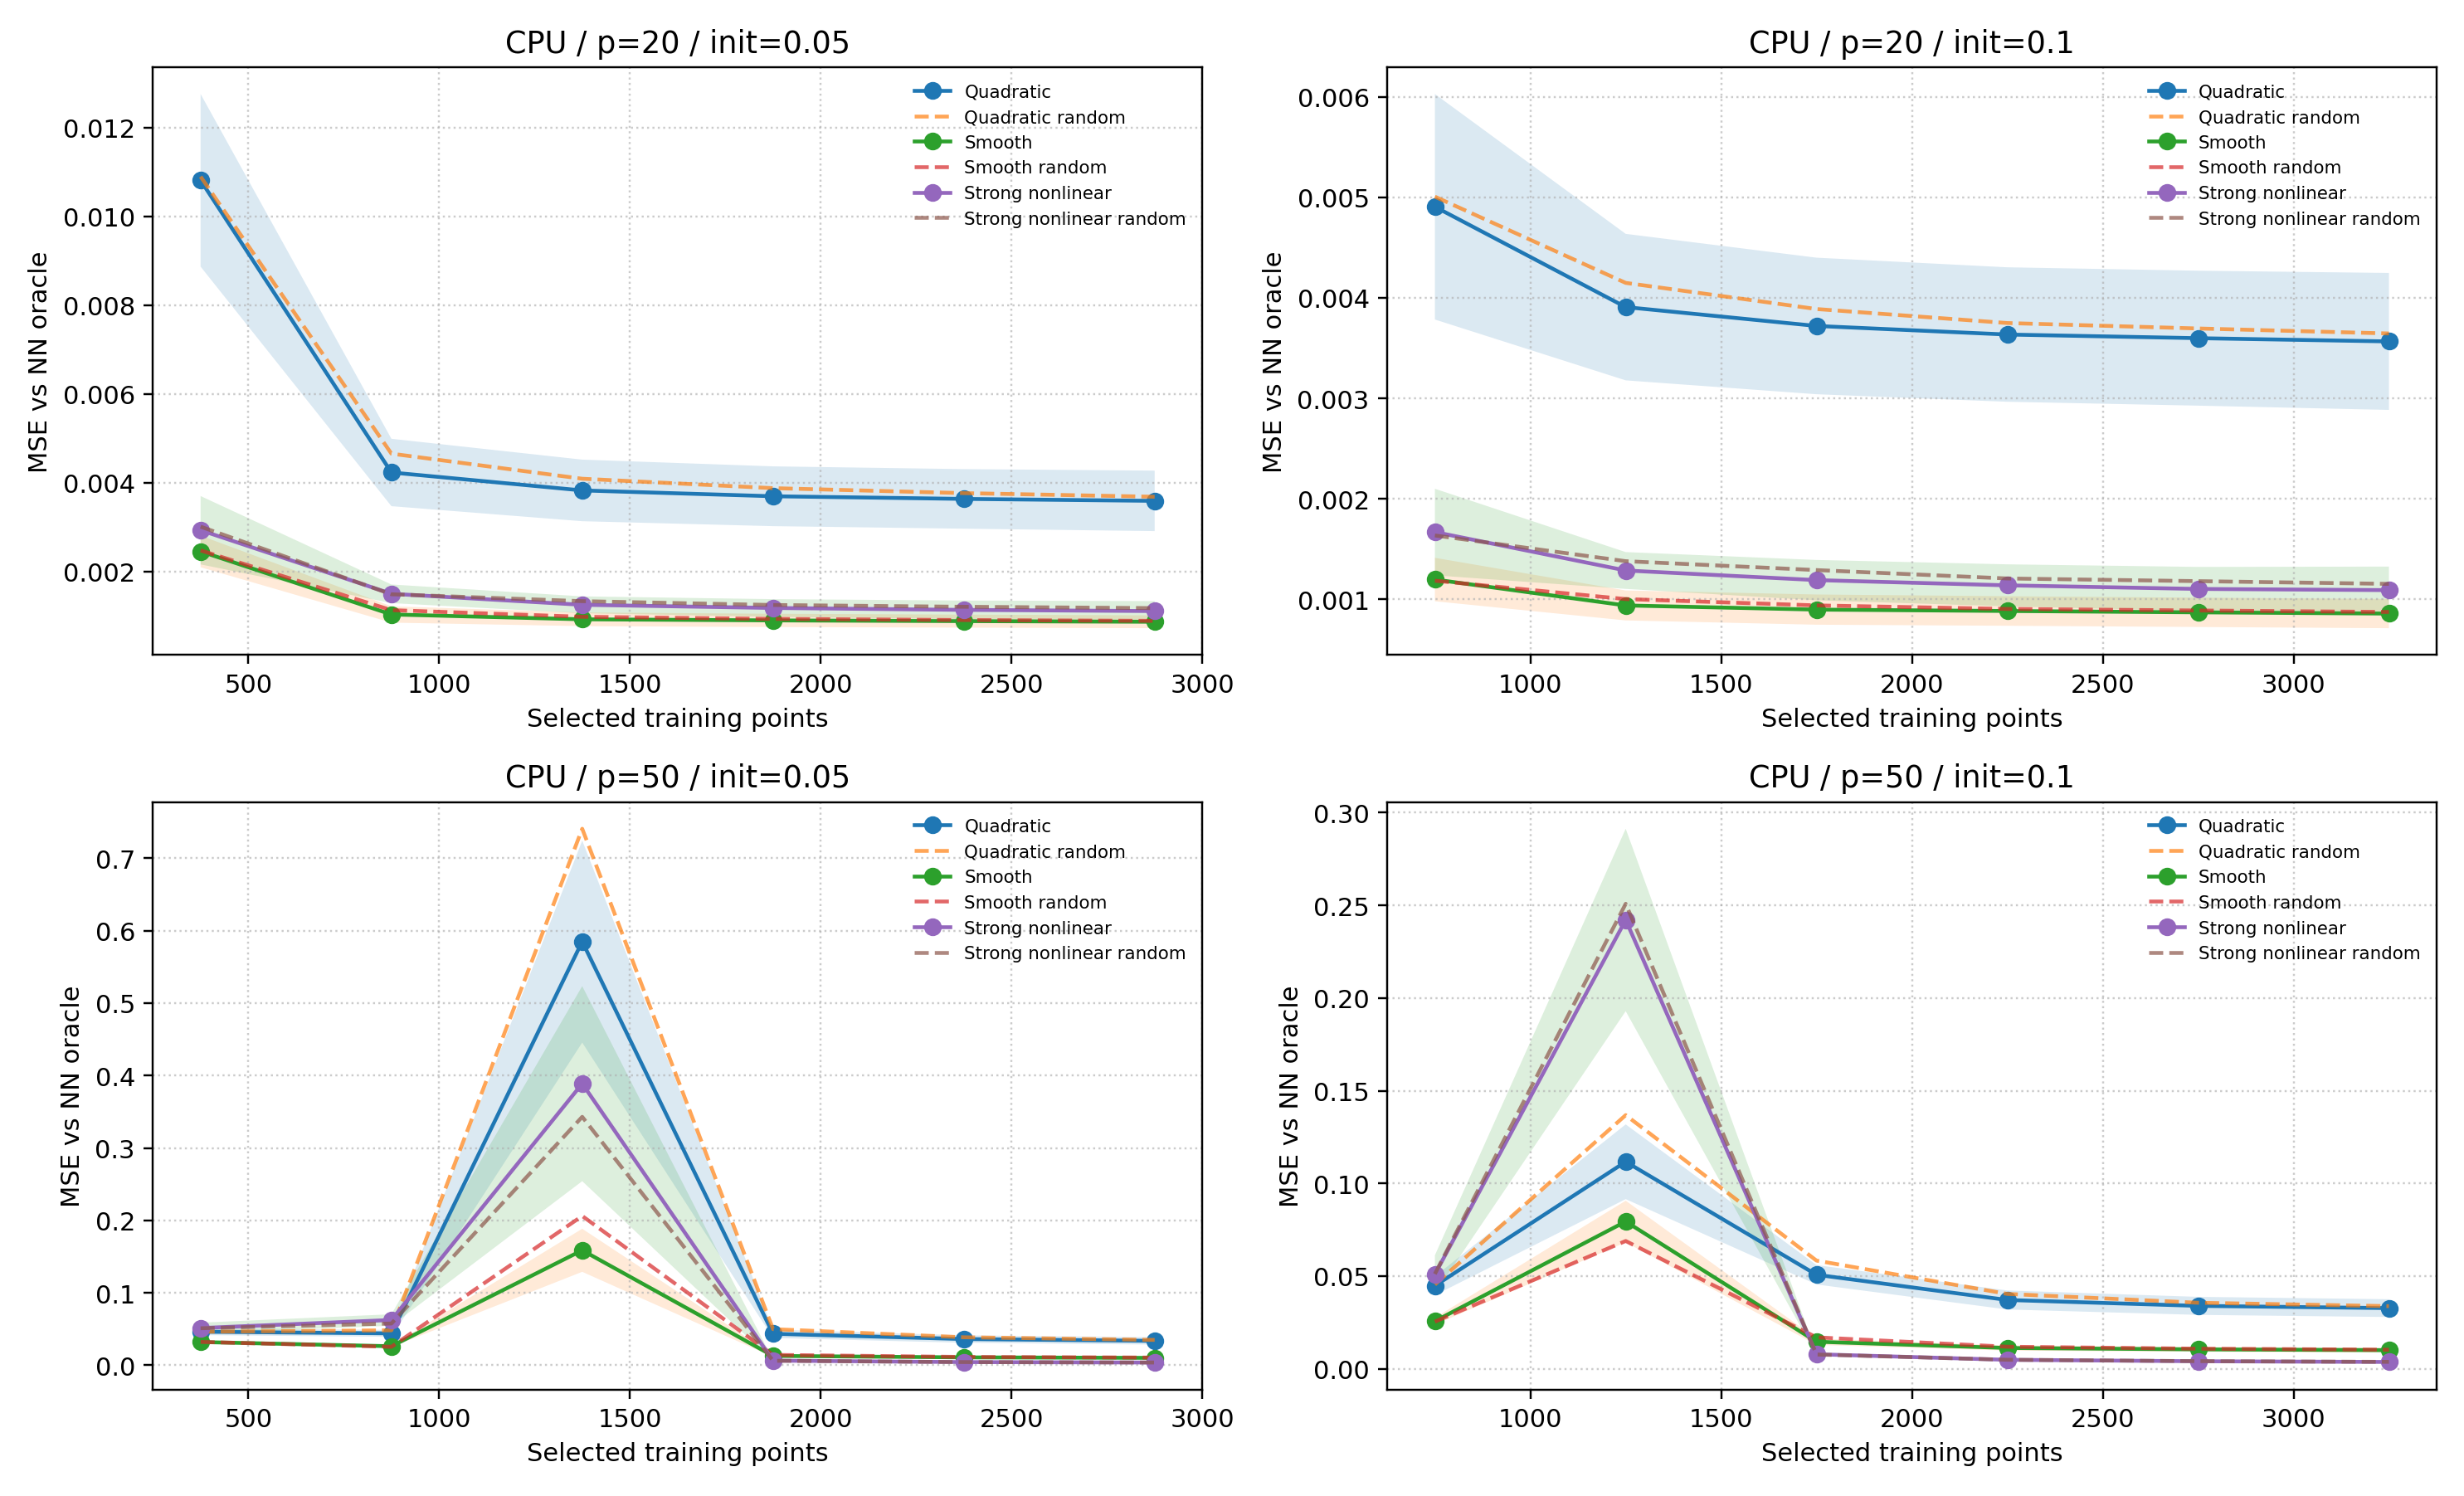
\includegraphics[width=0.92\textwidth]{figures/highdim_iter/paper_highdim_iter_dopt_cpu_mse_mean_ci.png}
\caption{CPU 实验中 D-optimal surrogate 与随机基准的 MSE 迭代曲线。}
\end{figure}

\begin{figure}[htbp]
\centering
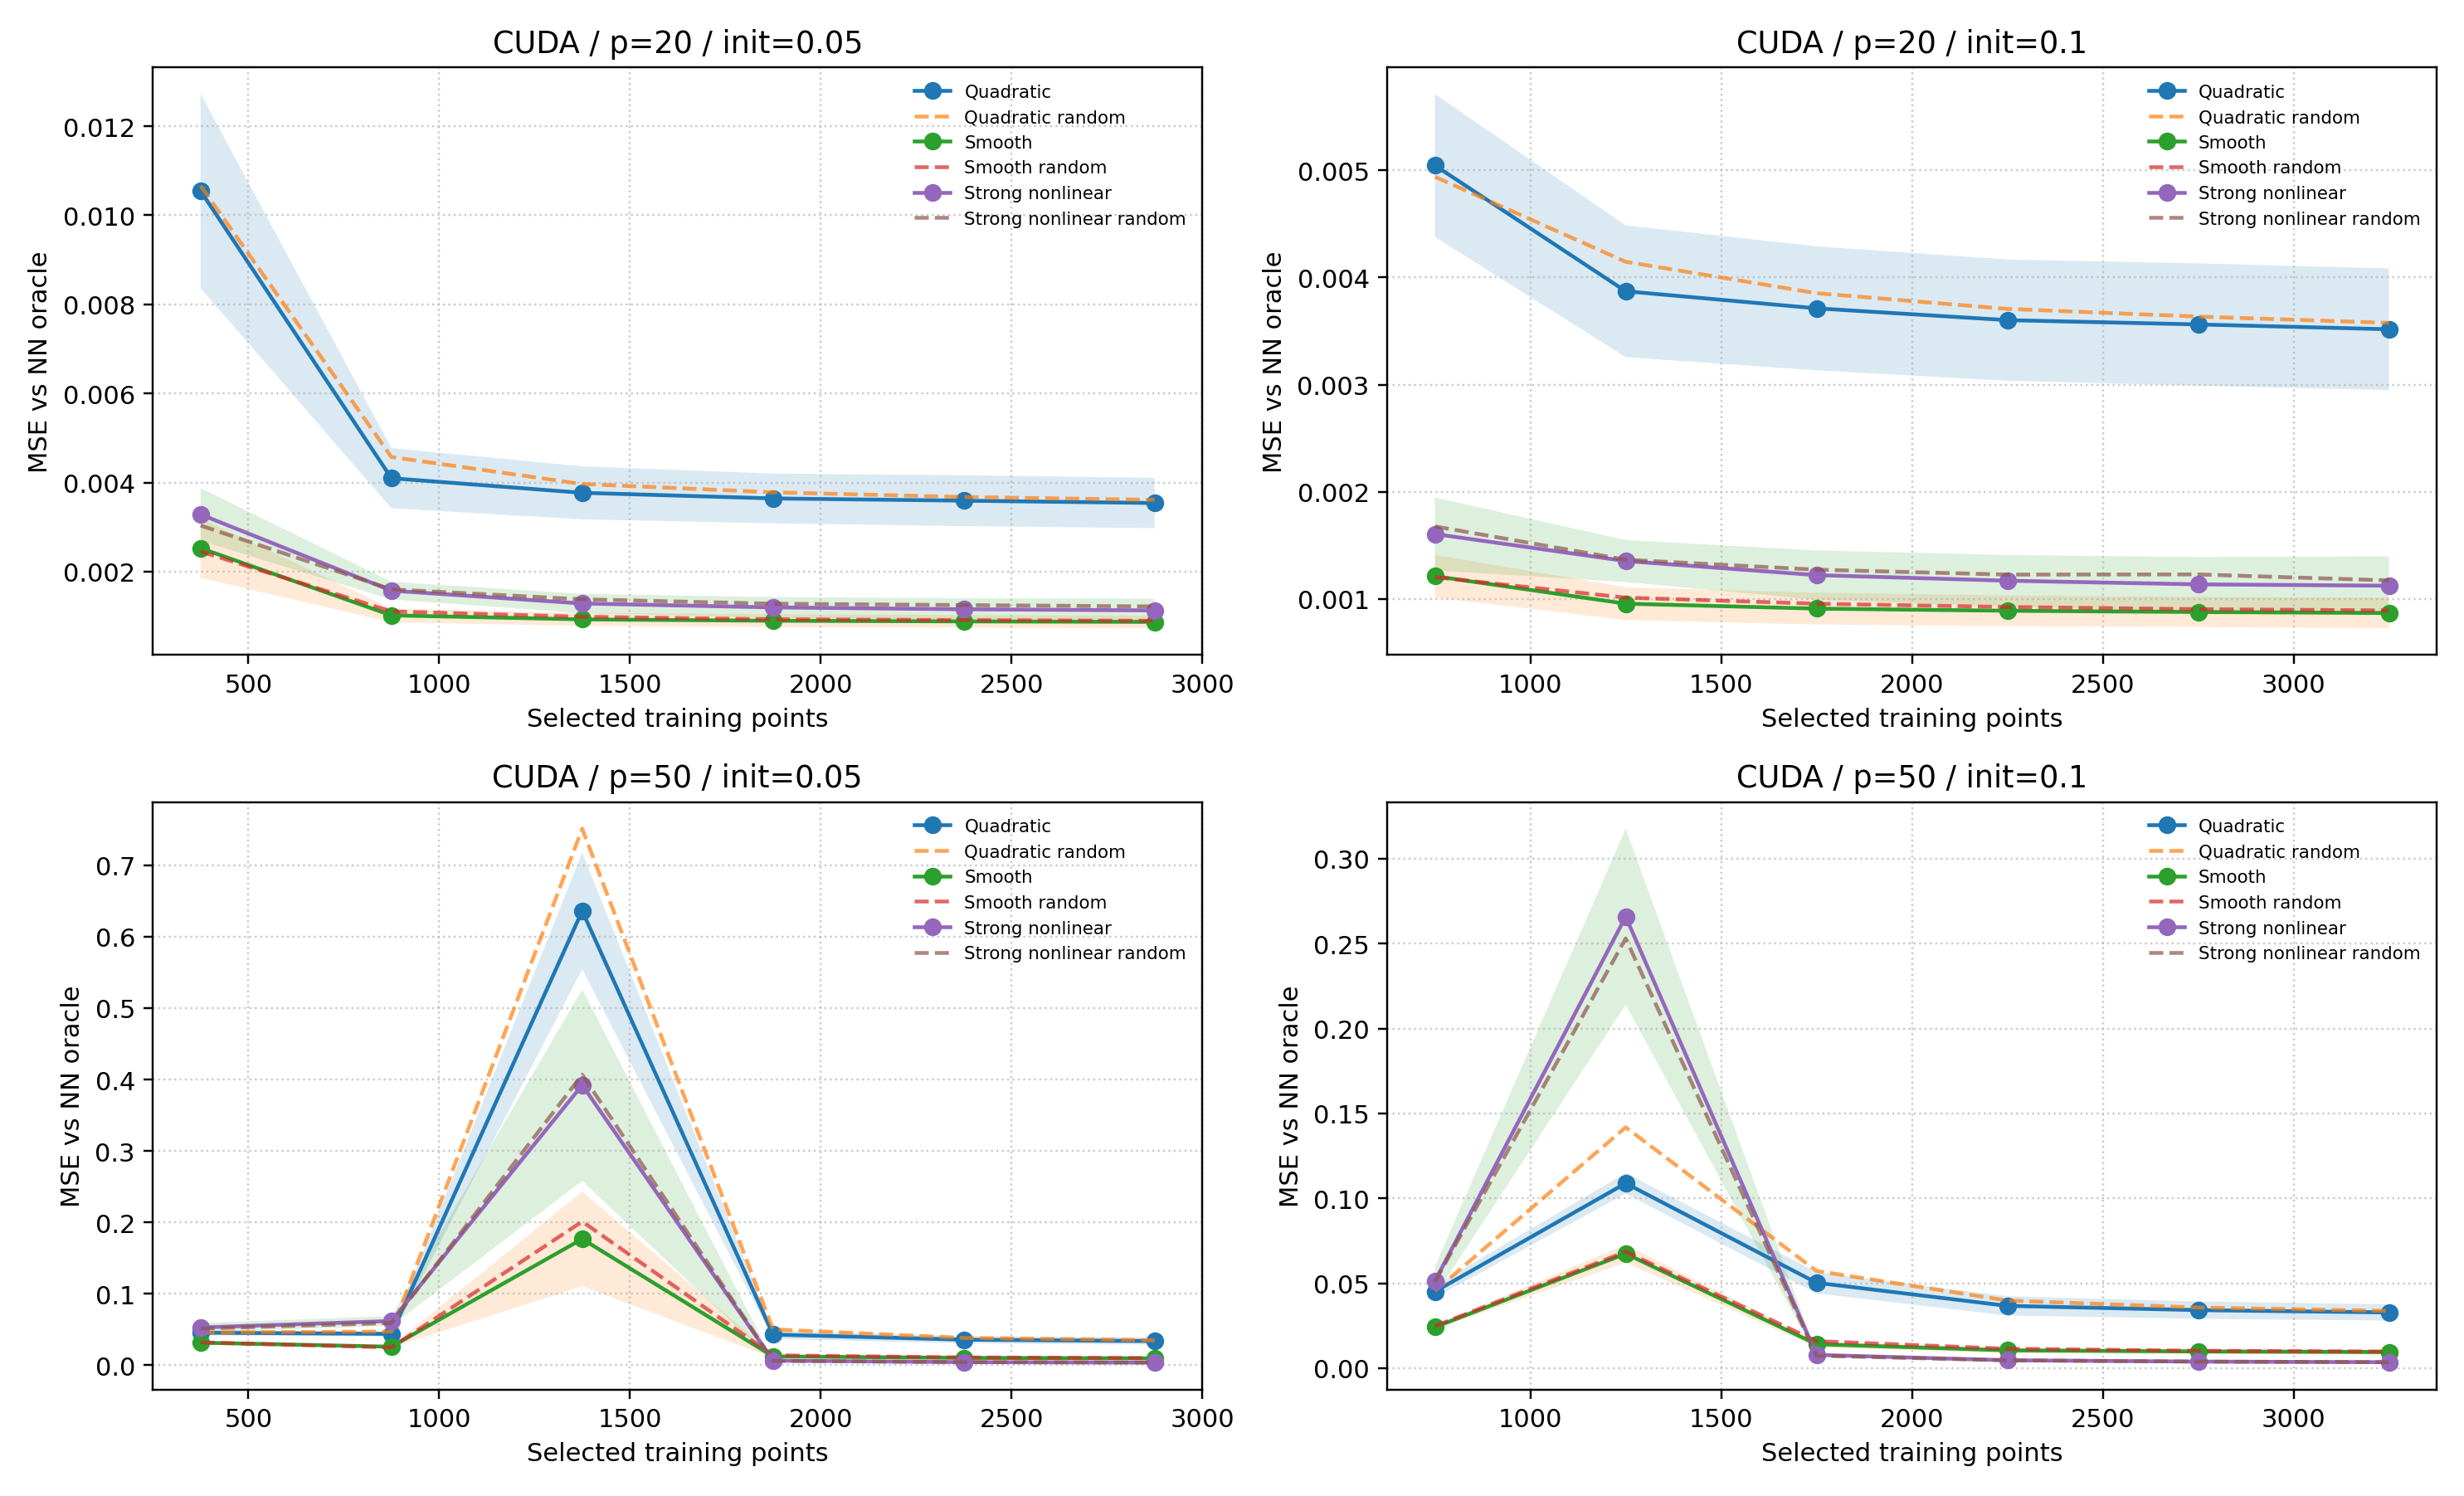
\includegraphics[width=0.92\textwidth]{figures/highdim_iter/paper_highdim_iter_dopt_cuda_mse_mean_ci.png}
\caption{CUDA 实验中 D-optimal surrogate 与随机基准的 MSE 迭代曲线。}
\end{figure}

\subsection{讨论}

\begin{itemize}
\item p=20 时二阶 FullPR 特征数较少，初始样本通常已超过特征数，因此 D-optimal 的收益较温和，但正收益比例高。
\end{itemize}

\begin{itemize}
\item p=50 时初始设计集更容易低于 FullPR 特征数，早期迭代出现更大波动；当升级数据集继续进入下一轮 D-optimal 后，误差逐步稳定。
\end{itemize}

\begin{itemize}
\item strong nonlinear 场景的置信区间明显更宽，说明当 NN oracle 的局部行为超出二阶 FullPR 表达能力时，D-optimal 仍能改善覆盖，但不能被解释为充分逼近 NN 的保证。
\end{itemize}

\begin{itemize}
\item CPU/GPU 的总体结论一致，说明结果不是单一设备偶然现象。
\end{itemize}

\end{document}